% Options for packages loaded elsewhere
\PassOptionsToPackage{unicode}{hyperref}
\PassOptionsToPackage{hyphens}{url}
%
\documentclass[
  man,floatsintext]{apa7}
\usepackage{amsmath,amssymb}
\usepackage{lmodern}
\usepackage{iftex}
\ifPDFTeX
  \usepackage[T1]{fontenc}
  \usepackage[utf8]{inputenc}
  \usepackage{textcomp} % provide euro and other symbols
\else % if luatex or xetex
  \usepackage{unicode-math}
  \defaultfontfeatures{Scale=MatchLowercase}
  \defaultfontfeatures[\rmfamily]{Ligatures=TeX,Scale=1}
\fi
% Use upquote if available, for straight quotes in verbatim environments
\IfFileExists{upquote.sty}{\usepackage{upquote}}{}
\IfFileExists{microtype.sty}{% use microtype if available
  \usepackage[]{microtype}
  \UseMicrotypeSet[protrusion]{basicmath} % disable protrusion for tt fonts
}{}
\makeatletter
\@ifundefined{KOMAClassName}{% if non-KOMA class
  \IfFileExists{parskip.sty}{%
    \usepackage{parskip}
  }{% else
    \setlength{\parindent}{0pt}
    \setlength{\parskip}{6pt plus 2pt minus 1pt}}
}{% if KOMA class
  \KOMAoptions{parskip=half}}
\makeatother
\usepackage{xcolor}
\usepackage{graphicx}
\makeatletter
\def\maxwidth{\ifdim\Gin@nat@width>\linewidth\linewidth\else\Gin@nat@width\fi}
\def\maxheight{\ifdim\Gin@nat@height>\textheight\textheight\else\Gin@nat@height\fi}
\makeatother
% Scale images if necessary, so that they will not overflow the page
% margins by default, and it is still possible to overwrite the defaults
% using explicit options in \includegraphics[width, height, ...]{}
\setkeys{Gin}{width=\maxwidth,height=\maxheight,keepaspectratio}
% Set default figure placement to htbp
\makeatletter
\def\fps@figure{htbp}
\makeatother
\setlength{\emergencystretch}{3em} % prevent overfull lines
\providecommand{\tightlist}{%
  \setlength{\itemsep}{0pt}\setlength{\parskip}{0pt}}
\setcounter{secnumdepth}{-\maxdimen} % remove section numbering
% Make \paragraph and \subparagraph free-standing
\ifx\paragraph\undefined\else
  \let\oldparagraph\paragraph
  \renewcommand{\paragraph}[1]{\oldparagraph{#1}\mbox{}}
\fi
\ifx\subparagraph\undefined\else
  \let\oldsubparagraph\subparagraph
  \renewcommand{\subparagraph}[1]{\oldsubparagraph{#1}\mbox{}}
\fi
\newlength{\cslhangindent}
\setlength{\cslhangindent}{1.5em}
\newlength{\csllabelwidth}
\setlength{\csllabelwidth}{3em}
\newlength{\cslentryspacingunit} % times entry-spacing
\setlength{\cslentryspacingunit}{\parskip}
\newenvironment{CSLReferences}[2] % #1 hanging-ident, #2 entry spacing
 {% don't indent paragraphs
  \setlength{\parindent}{0pt}
  % turn on hanging indent if param 1 is 1
  \ifodd #1
  \let\oldpar\par
  \def\par{\hangindent=\cslhangindent\oldpar}
  \fi
  % set entry spacing
  \setlength{\parskip}{#2\cslentryspacingunit}
 }%
 {}
\usepackage{calc}
\newcommand{\CSLBlock}[1]{#1\hfill\break}
\newcommand{\CSLLeftMargin}[1]{\parbox[t]{\csllabelwidth}{#1}}
\newcommand{\CSLRightInline}[1]{\parbox[t]{\linewidth - \csllabelwidth}{#1}\break}
\newcommand{\CSLIndent}[1]{\hspace{\cslhangindent}#1}
\ifLuaTeX
\usepackage[bidi=basic]{babel}
\else
\usepackage[bidi=default]{babel}
\fi
\babelprovide[main,import]{english}
% get rid of language-specific shorthands (see #6817):
\let\LanguageShortHands\languageshorthands
\def\languageshorthands#1{}
% Manuscript styling
\usepackage{upgreek}
\captionsetup{font=singlespacing,justification=justified}

% Table formatting
\usepackage{longtable}
\usepackage{lscape}
% \usepackage[counterclockwise]{rotating}   % Landscape page setup for large tables
\usepackage{multirow}		% Table styling
\usepackage{tabularx}		% Control Column width
\usepackage[flushleft]{threeparttable}	% Allows for three part tables with a specified notes section
\usepackage{threeparttablex}            % Lets threeparttable work with longtable

% Create new environments so endfloat can handle them
% \newenvironment{ltable}
%   {\begin{landscape}\centering\begin{threeparttable}}
%   {\end{threeparttable}\end{landscape}}
\newenvironment{lltable}{\begin{landscape}\centering\begin{ThreePartTable}}{\end{ThreePartTable}\end{landscape}}

% Enables adjusting longtable caption width to table width
% Solution found at http://golatex.de/longtable-mit-caption-so-breit-wie-die-tabelle-t15767.html
\makeatletter
\newcommand\LastLTentrywidth{1em}
\newlength\longtablewidth
\setlength{\longtablewidth}{1in}
\newcommand{\getlongtablewidth}{\begingroup \ifcsname LT@\roman{LT@tables}\endcsname \global\longtablewidth=0pt \renewcommand{\LT@entry}[2]{\global\advance\longtablewidth by ##2\relax\gdef\LastLTentrywidth{##2}}\@nameuse{LT@\roman{LT@tables}} \fi \endgroup}

% \setlength{\parindent}{0.5in}
% \setlength{\parskip}{0pt plus 0pt minus 0pt}

% Overwrite redefinition of paragraph and subparagraph by the default LaTeX template
% See https://github.com/crsh/papaja/issues/292
\makeatletter
\renewcommand{\paragraph}{\@startsection{paragraph}{4}{\parindent}%
  {0\baselineskip \@plus 0.2ex \@minus 0.2ex}%
  {-1em}%
  {\normalfont\normalsize\bfseries\itshape\typesectitle}}

\renewcommand{\subparagraph}[1]{\@startsection{subparagraph}{5}{1em}%
  {0\baselineskip \@plus 0.2ex \@minus 0.2ex}%
  {-\z@\relax}%
  {\normalfont\normalsize\itshape\hspace{\parindent}{#1}\textit{\addperi}}{\relax}}
\makeatother

% \usepackage{etoolbox}
\makeatletter
\patchcmd{\HyOrg@maketitle}
  {\section{\normalfont\normalsize\abstractname}}
  {\section*{\normalfont\normalsize\abstractname}}
  {}{\typeout{Failed to patch abstract.}}
\patchcmd{\HyOrg@maketitle}
  {\section{\protect\normalfont{\@title}}}
  {\section*{\protect\normalfont{\@title}}}
  {}{\typeout{Failed to patch title.}}
\makeatother

\usepackage{xpatch}
\makeatletter
\xapptocmd\appendix
  {\xapptocmd\section
    {\addcontentsline{toc}{section}{\appendixname\ifoneappendix\else~\theappendix\fi\\: #1}}
    {}{\InnerPatchFailed}%
  }
{}{\PatchFailed}
\keywords{COVID-19, well-being, social media, news use, panel study.}
\usepackage{lineno}

\linenumbers
\usepackage{csquotes}
\makeatletter
\renewcommand{\paragraph}{\@startsection{paragraph}{4}{\parindent}%
  {0\baselineskip \@plus 0.2ex \@minus 0.2ex}%
  {-1em}%
  {\normalfont\normalsize\bfseries\typesectitle}}

\renewcommand{\subparagraph}[1]{\@startsection{subparagraph}{5}{1em}%
  {0\baselineskip \@plus 0.2ex \@minus 0.2ex}%
  {-\z@\relax}%
  {\normalfont\normalsize\bfseries\itshape\hspace{\parindent}{#1}\textit{\addperi}}{\relax}}
\makeatother
\usepackage{endnotes}
\setlength{\parskip}{0em}
\raggedbottom
\note{\clearpage}

\ifLuaTeX
  \usepackage{selnolig}  % disable illegal ligatures
\fi
\IfFileExists{bookmark.sty}{\usepackage{bookmark}}{\usepackage{hyperref}}
\IfFileExists{xurl.sty}{\usepackage{xurl}}{} % add URL line breaks if available
\urlstyle{same} % disable monospaced font for URLs
\hypersetup{
  pdftitle={No meaningful effects of COVID-19 related social media use on well-being},
  pdfauthor={Tobias Dienlin1},
  pdflang={en-EN},
  pdfkeywords={COVID-19, well-being, social media, news use, panel study.},
  hidelinks,
  pdfcreator={LaTeX via pandoc}}

\title{No meaningful effects of COVID-19 related social media use on well-being}
\author{Tobias Dienlin\textsuperscript{1}}
\date{}


\shorttitle{COVID-19 related social media use and well-being}

\authornote{

Tobias Dienlin, Department of Communication, University of Vienna.

Correspondence concerning this article should be addressed to Tobias Dienlin, University of Vienna, Department of Communication, 1090 Vienna, Austria. E-mail: \href{mailto:tobias.dienlin@univie.ac.at}{\nolinkurl{tobias.dienlin@univie.ac.at}}

}

\affiliation{\vspace{0.5cm}\textsuperscript{1} University of Vienna}

\note{

Preprint submitted for publication. Please cite carefully.

}

\abstract{%
In times of crisis such as the Corona pandemic citizens need to stay informed about recent events, the latest political decisions, or mandatory protection measures. To this end, many people use various types of media, and increasingly social media. However, because social media are particularly engaging, some find it hard to disconnect and cannot stop `doomscrolling'. In this preregistered study, I investigate whether using social media for COVID-19 related reasons affects psychological well-being. To answer this question I analyzed data from the Austrian Corona Panel Project, which consists of 24 waves with overall 3,018 participants. I ran three random effects within between models, controlling for several stable and varying confounders. Results showed that the effects of COVID-19 related social media use on well-being were very small, arguably too small to matter. The findings suggest that fears that social media use during times of crisis impairs well-being are likely to be unfounded.
}



\begin{document}
\maketitle

During the COVID-19 pandemic it was critical to stay informed regarding the latest developments.
How dangerous is the virus?
In what region is it spreading?
How is it transmitted? What are the current safety regulations?
To obtain relevant information, many people heavily relied on social media, which were at an all time high (Statista, 2021).

Some actually could not stop using social media to learn about COVID-19 related news.
A new phenomenon termed ``doomscrolling'' emerged.
Many users were glued to their screens and found it hard to pursue other relevant activities such as working, taking a break, or even looking after their children (Klein, 2021).
In the media it was hence increasingly asked whether using social media for COVID-19 related reasons would, next to all other stressors, create an additional burden on mental health (Sandstrom et al., 2021).
Although research has begun addressing this question (Bendau et al., 2021; Bradley \& Howard, 2021; Choi \& Choung, 2021; Dörnemann et al., 2021; Eden et al., 2020; Guazzini et al., 2022; Latikka et al., 2022; Liu \& Tong, 2020; Riehm et al., 2020; Sewall et al., 2021; Stainback et al., 2020; Yue et al., 2022), it still largely unknown if COVID-19 related social media use during the pandemic has had a meaningful impact on well-being.
By analyzing large-scale panel data from Austria and by focusing on intra-individual causal effects, this study aims to answer to this question.

\hypertarget{understanding-well-being-and-media-use}{%
\subsection{Understanding Well-being and Media Use}\label{understanding-well-being-and-media-use}}

This study investigates how different \emph{facets} of well-being are affected by different \emph{types} and different \emph{channels} of communication (Meier \& Reinecke, 2020).
Building on the typology of subjective well-being (Diener et al., 2018), three different well-being facets are analyzed: life satisfaction, positive affect, and negative affect.
Because effects of social media depend on how they are used (Verduyn et al., 2015), I further distinguish three types of use and five popular channels.
The types of use include reading, posting, and liking and sharing COVID-19 related posts.
In doing so, this study analyzes social media use focused on COVID-19 related content, which includes posting thoughts about the pandemic, reading posts and comments, or retweeting COVID-19 related news.
The five channels to be investigated are Facebook, Twitter, Instagram, WhatsApp, and YouTube, which at the time ranked among the most popular social media services in Austria.

How could the various types and channels of COVID-19 related social media use affect well-being?
According to the set-point theory, well-being is surprisingly stable (Lykken, 1999).
Although specific events such as marriage or salary can have significant impacts on well-being, in most cases effects are only short-term, with well-being after some time routinely returning to prior levels (Sheldon \& Lucas, 2014).
Only very specific factors such as unemployment, disability, or death can cause long-term changes in well-being (Lucas, 2007).
Can media use be such a factor?
Current literature overviews suggest no:
Although social media use on average decreases well-being, the effects are small (Meier \& Reinecke, 2020).
In addition, the effects of media use differ across individuals and types of content (Valkenburg \& Peter, 2013).
Whereas for some users social media are more beneficial, for others they are more harmful.
For example, in one study it was estimated that roughly one quarter of all users experienced negative effects, another quarter positive effects, while for the rest the effects were neutral (Beyens et al., 2021).
This finding is aligned with the Differential Susceptibility to Media Effects Model:
Although there is substantial \emph{variation} of media effects for individual users, there are both negative and positive aspects, leading to small effects on average (Valkenburg \& Peter, 2013)---as confirmed by several literature overviews (Dienlin \& Johannes, 2020; Huang, 2017; Meier \& Reinecke, 2020; Orben, 2020).

Why are the effects of social media use on well-being small on average?
Using Social media is ambivalent.
It can impair well-being when causing embarrassment, stress, or disinformation, and it can improve well-being when providing connectedness, information, or entertainment (Büchi, 2021).
Although social media are often associated with negative outcomes, there are a large number of positive effects, which either offset or at least significantly reduce negative outcomes.
Positive outcomes encompass finding relevant information; maintaining and fostering relationships; expressing one's personality; or entertaining oneself (e.g., Pelletier et al., 2020).
Negative effects include distraction; displacement of other meaningful activities; consumption of shallow, misleading or challenging content; or negative social comparisons (e.g., Meier \& Krause, 2022).
People are much more likely to use media that offer plentiful benefits (Katz et al., 1973).
Users implicitly learn what media help them regulate their mood and thereby well-being (Zillmann, 1988).
Given the ubiquitous use of social media, the many benefits they offer, plus the general and implicit competence to use media that foster mood management, it is hence unlikely that the effects of social media use on well-being are profusely negative.

There is still little empirical research on how well-being is affected by social media use that is focused on COVID-19 specifically.
Results are mixed.
When browsing social media for COVID-19 related news, many users reported being captivated to such an extent they could not stop using social media (Klein, 2021).
In a study with 1,131 residents from Wuhan in China, people who spent more time in quarantine also spent more time on social media (Yue et al., 2022).
Those who spent more time on social media also engaged in more upward social comparison, which was related to increased levels of stress.
People who used social media as a primary source of information reported on average ``significantly more unspecific anxiety and depression {[}\ldots{]} and significantly more specific COVID-19 related anxiety symptoms'' (Bendau et al., 2021, p. 288).
Eden et al. (2020) analyzed how 425 US college students used media during the first wave of the pandemic, finding both positive and negative relations with well-being.
In a large-scale study with 11,537 respondents from the US, increased COVID-19-related media consumption was related to more psychological distress (Stainback et al., 2020).
A four-wave panel study with 384 young adults from the U.S. analyzed the effects of general digital technology use during the pandemic on mental health, finding that digital technology did not have significant effects on mental health (Sewall et al., 2021; for a similar study with comparable results, see Bradley \& Howard, 2021).
A study with 2.057 respondents from Italy reported that during the pandemic virtual community and social connectedness increased (Guazzini et al., 2022).
In a study with 735 participants from Finland, levels of loneliness were stable during the pandemic, and people who engaged more on social media experienced less loneliness (Latikka et al., 2022).
Together, the literature is mixed, showing both positive and negative affects of social media use focused on or during COVID-19 on well-being (see also Dörnemann et al., 2021; Liu \& Tong, 2020; Riehm et al., 2020).

In conclusion, these mixed empirical results, together with the observation that social media effects on well-being are very small in general, I expect that COVID-19 related communication on social media does not affect well-being in a meaningful or relevant way.

\begin{quote}
Hypothesis: The within-person effects of all types of COVID-19 related social media use on all types of well-being indicators---while controlling for several stable and varying covariates such as sociodemographic variables and psychological dispositions---will be trivial.
\end{quote}

\hypertarget{method}{%
\section{Method}\label{method}}

\hypertarget{preregistration}{%
\subsection{Preregistration}\label{preregistration}}

The hypotheses, the sample, the measures, the analyses, and the inference criteria (SESOI, \emph{p}-value) were preregistered on the Open Science Framework, accessible here: \url{https://osf.io/87b24/?view_only=b2289b6fec214fa88ee75a18d45c18f3}.
Because in this study I analyze data from an already existing large-scale data set, the preregistration was done prior to accessing the data.
The preregistration was designed on the basis of the panel documentation online (Kittel et al., 2020).
In some cases, it was impossible to execute the analyses as I had originally planned, for example because some properties of the variables only became apparent when seeing the actual data.
The most relevant deviations are reported below, and a complete list of all changes can be found in the online \href{https://XMtRA.github.io/Austrian_Corona_Panel_Project}{companion website} (\url{https://XMtRA.github.io/Austrian_Corona_Panel_Project}).

\hypertarget{sample}{%
\subsection{Sample}\label{sample}}

The data come from the Austrian Corona Panel Project (Kittel et al., 2021), which is a large-scale standalone panel study.
The data are hosted on AUSSDA, are publicly available here (\url{https://doi.org/10.11587/28KQNS}), and consist of 32 waves.
The study was conducted between March 2020 and June 2022, and data collection is now finished.
Between March 2020 and July 2020, the intervals between waves were weekly and afterward monthly.
Each wave consists of at least 1,500 respondents.
The sample size was \emph{N} = 3,485, with overall 111,520 observations.
Panel mortality was compensated through a continuous re-acquisition of new participants.
Participants were sampled from a pre-existing online access panel provided by the company Marketagent, Austria.
Panel members were incentivized with 180 credit points for each wave of the study.

Achieved via quota sampling, the sample matched the Austrian population in terms of age, gender, region/state, municipality size, and educational level.
In order to participate in the study, the respondents needed to be Austrian residents and had to be at least 14 years of age.
All respondents needed to have access to the internet (via computer or mobile devices such as smartphones or tablets).
Ethical review and approval was not required for the study in accordance with the local legislation and institutional requirements.
The participants provided their written informed consent to participate in this study.
The average age was 41 years, 49 percent were male, 14 percent had a University degree, and 5 percent were currently unemployed.

\hypertarget{smallest-effect-size-of-interest}{%
\subsection{Smallest Effect Size of Interest}\label{smallest-effect-size-of-interest}}

Testing the hypothesis necessitates defining what is considered a ``trivial effect size''.
Being a normative question, finding a clear, single, or unanimous answer is impossible.
However, it is still necessary and helpful to work toward a plausible benchmark.
I suggest the following SESOI for this research question:

\begin{quote}
SESOI: If a heavy user of COVID-19 related social media news suddenly \emph{stops} using social media altogether, this should have a \emph{noticeable} impact on their overall well-being.
\end{quote}

What does this mean practically and how can it be operationalized?
In this study, COVID-19 related social media use was measured on a 5-point scale, ranging from 1 = \emph{never} to 5 = \emph{several times a day}. Thus, a change of four units in social media use (e.g., a complete stop) should correspond to a noticeable change in well-being.
What is a noticeable change in well-being?
According to Norman et al. (2003), people can reliably distinguish seven levels of satisfaction with health.
So if satisfaction is measured on a 7-point scale, a four unit change in social media use should result in a one unit change in life satisfaction.

In this study, life satisfaction was measured on an 11-point scale.
If people can reliably differentiate 7 levels, this corresponds to 11 / 7 = 1.57 unit change on an 11-point scale.
Hence, a four-point change in media use (e.g., a complete stop) should result in a 1.57-point change in life satisfaction.
In a statistical regression analysis, \emph{b} estimates the change in the dependent variable if the independent variable increases by one point.
For life satisfaction, we would therefore define a SESOI of \emph{b} = 1.57 / 4 = 0.39.
For positive or negative affect, which was measured on a 5-point scale, our SESOI would be \emph{b} = 0.71 / 4 = 0.18.
Because we are agnostic as to whether the effects are positive or negative, the null region includes both negative and positive effects.
Finally, in order not to exaggerate precision and to be less conservative, these numbers are reduced to nearby thresholds.\footnote{Note that other researchers also decreased or recommended decreasing thresholds for effect sizes when analyzing within-person or cumulative effects (Beyens et al., 2021; Funder \& Ozer, 2019).}
Together, this leads to a null region ranging from \emph{b} = -.30 to \emph{b} = .30 for life satisfaction, and \emph{b} = -.15 to \emph{b} = .15 for positive and negative affect.

The hypothesis is analyzed using the interval testing approach as proposed by Dienes (2014).
To illustrate, if the 95\% confidence interval falls completely within the null-region (e.g., \emph{b} = -.02, {[}95\% CI: -.12, .08{]}), the hypothesis that the effect is trivial is supported.
If the confidence interval and the null region overlap (e.g., \emph{b} = -.22, {[}95\% CI: -.27, -.17{]}), the hypothesis is not supported and the results are considered inconclusive, while a meaningful negative effect is rejected.
If the confidence interval falls completely outside of the null-region (e.g., \emph{b} = -.40, {[}95\% CI: -.45, -.35{]}), the hypothesis is rejected and the existence of a meaningful positive effect is supported.
For an illustration, see Figure \ref{fig:sesoi}.

\begin{figure}
\centering
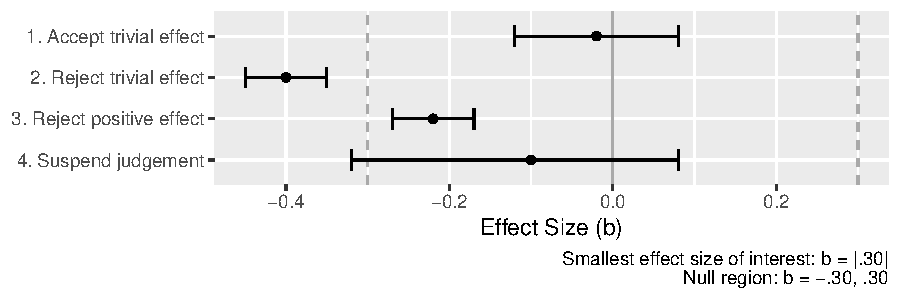
\includegraphics{manuscript_files/figure-latex/sesoi-1.pdf}
\caption{\label{fig:sesoi}Using confidence intervals to test a null region. In this study, a trivial effect of social media use on life satisfaction is defined as ranging from b = -.30 to b = .30}
\end{figure}

\hypertarget{data-analysis}{%
\subsection{Data Analysis}\label{data-analysis}}

\hypertarget{causality}{%
\subsubsection{Causality}\label{causality}}

When using longitudinal designs to analyze causality, it is important to (a) focus on within-person effects (Hamaker, 2014); to (b) control for confounders (Rohrer \& Murayama, 2021); and to (c) test a plausible interval between measures (Dormann \& Griffin, 2015).
To elaborate, in non-experimental designs it makes much sense to analyze causal effects from an internal, within-person perspective (Hamaker, 2014).
If a specific person changes their media diet, we need to measure how this behavior affects their well-being.
Between-person comparisons from longitudinal data cannot provide such insights (Lucas, 2022).
To test the hypothesis, I thus consider only the within-person effects.

Second, to identify confounders we should control for variables that affect both media use and well-being, which helps isolate the actual effect of social media use on well-being (Rohrer, 2018).
Because we are adopting a within-person perspective, we need to implement \emph{time-varying} confounders (Rohrer \& Murayama, 2021).
And because we are determining the \emph{overall} causal effect, we need to make sure \emph{not} to control for mediating variables (Rohrer, 2018), for doing so would bias our assessment of the causal effect.
In this study, I hence preregistered to control for the following variables, which either have already been shown or are very likely to affect both social media use and well-being, and which also are not mediators:
gender, age, education, Austria country of birth, Austria country of birth of parents, residency Vienna, text-based news consumption, video-based news consumption, household size, health, living space, access to garden, access to balcony, employment, work hours per week, being in home-office, household income, outdoor activities, satisfaction with democracy, disposition to take risks, and locus of control.

Finally, one precondition of causality is temporal order and finding a plausible interval (Dormann \& Griffin, 2015).
If variables are stable, longer intervals are needed; if they fluctuate, shorter intervals are required.
In the case of well-being, we need shorter intervals for the more fluctuating positive and negative affect, and longer ones for the more stable life satisfaction (Dienlin \& Johannes, 2020).
Using social media can have instant effects on mood (Marciano et al., 2022).
Effects on life satisfaction often take longer to manifest, for example because media use leads to actual changes in specific behaviors, which then in turn affect life satisfaction (Dienlin et al., 2017).
In this study, I hence analyze how using social media during the last week affected positive and negative affect during the same week.
In other words, if people during the last week engaged in more COVID-19 related social media use than usual, did they feel better or worse during that week than usual?
For life satisfaction, I implemented a longer interval.
If people during the last week used COVID-19 related social media more than they usually do, were they at the end of the week more or less satisfied with their lives than they usually are?
I hence analyze if when a person changes their social media diet, are there (a) \emph{simultaneous} changes in their affect and (b) \emph{subsequent} changes in their life satisfaction?
These relations will be controlled for varying confounders, which fosters a causal interpretation.

\hypertarget{statistical-model}{%
\subsubsection{Statistical model}\label{statistical-model}}

The hypothesis was analyzed using random effect within-between models (REWB, Bell et al., 2019).
Altogether three models were run, one for each dependent variable.
The data were hierarchical, and responses were separately nested in participants and waves (i.e., participants and waves were implemented as random effects).
Nesting in participants allowed to separate between-person relations from within-person effects.
Nesting in waves allowed to control for general exogenous developments, such as general decreases in well-being in the population, for example due to lockdown measures.
Thus, there was no need additionally to control for specific phases or measures of the lockdown.
Predictors were modeled as fixed effects.
They included social media communication types and channels, separated into within and between-person factors, as well as stable and varying covariates.
All predictors were included simultaneously in each of the three models.

The factorial validity of the scales were tested with confirmatory factor analyses (CFA).
Because Mardia's test showed that the assumption of multivariate normality was violated, I used the more robust Satorra-Bentler scaled and mean-adjusted test statistic (MLM) as estimator.
Mean scores were used for positive and negative affect.
Missing responses were imputed using multiple imputation with predictive mean matching (five iterations, five data-sets), including categorical variables.
All variables were imputed except the social media use measures, as they were not collected on each wave.
All variables included in the analyses presented here were used to impute missing data.

\hypertarget{robustness-checks}{%
\subsubsection{Robustness-checks}\label{robustness-checks}}

To find out whether the inferences were robust across plausible but subordinate analyses, I conducted additional exploratory analyses.
I reran the analyses (a) with additional not-preregistered covariates such as trust in media or government, (b) without covariates, (c) with single imputation, and (d) without imputation.
For more information on the analyses, a complete documentation of the models and results, and all additional analyses, see \href{https://XMtRA.github.io/Austrian_Corona_Panel_Project}{companion website}.

\hypertarget{measures}{%
\subsection{Measures}\label{measures}}

For the variables' means, range, and variance, see Table \ref{tab:tab-descriptives}.
For a complete list of all items and item characteristics, see \href{https://XMtRA.github.io/Austrian_Corona_Panel_Project}{companion website}.

\hypertarget{well-being}{%
\subsubsection{Well-being}\label{well-being}}

Life satisfaction was measured with the item ``All things considered, how satisfied are you with your life as a whole nowadays?'', which comes from the European Social Survey (European Social Survey, 2021).
The response options ranged from 0 (\emph{extremely dissatisfied}) to 10 (\emph{extremely satisfied}).

To capture positive affect, respondents were asked how often in the last week they felt (a) calm and relaxed, (b) happy, and (c) full of energy (World Health Organization, 1998).
The response options were 1 (\emph{never}), 2 (\emph{on some days}), 3 (\emph{several times per week}), 4 (\emph{almost every day}), and 5 (\emph{daily}).
The scale showed good factorial fit, \(\chi^2\)(62) = 67.03, \emph{p} = .309, CFI = 1.00, RMSEA \textless{} .01, 90\% CI {[}\textless{} .01, .02{]}, SRMR = .01.
Reliability was high, \(\omega\) = .85.

For negative affect, respondents were asked how often in the last week they felt (a) lonely, (b) aggravated, (c) so depressed, that nothing could lift you up, (d) very nervous, (e) anxious, and (h) glum and sad (World Health Organization, 1998).
The response options were 1 (\emph{never}), 2 (\emph{on some days}), 3 (\emph{several times per week}), 4 (\emph{almost every day}), and 5 (\emph{daily}).
The scale showed good factorial fit, \(\chi^2\)(443) = 3810.53, \emph{p} \textless{} .001, CFI = .98, RMSEA = .07, 90\% CI {[}.07, .08{]}, SRMR = .03.
Reliability was high, \(\omega\) = .91.

All three variables were measured on each wave.

\hypertarget{covid-19-related-social-media-use}{%
\subsubsection{COVID-19 related social media use}\label{covid-19-related-social-media-use}}

COVID-19 related social media use focused on communication types was measured with the three dimensions of (a) reading, (b) liking and sharing, and (c) posting.
The items come from Wagner et al. (2018) and were adapted for the context of this study.
The general introductory question was ``How often during the last week have you engaged in the following activities on social media?''.
The three items were ``Reading the posts of others with content on the Coronavirus'', ``When seeing posts on the Coronavirus, I clicked `like', `share' or `retweet'\,'', ``I myself wrote posts on the Coronavirus on social media.''
Answer options were 1 (\emph{several times per day}), 2 (\emph{daily}), 3 (\emph{several times per week}), 4 (\emph{weekly}), 5 (\emph{never}).
The items were inverted for the analyses.

COVID-19 related social media use focused on channels was measured with five variables from Wagner et al. (2018), adapted for this study.
The general introductory question was ``How often in the last week have you followed information related to the Corona-crisis on the following social media?''
The five items were (a) Facebook, (b) Twitter, (c) Instagram, (d) Youtube, and (e) WhatsApp.
Again, the answer options were 1 (\emph{several times per day}), 2 (\emph{daily}), 3 (\emph{several times per week}), 4 (\emph{weekly}), 5 (\emph{never}).
Again, the items were inverted for the analyses.

Social media use was measured for all participants on waves 1, 2, 8, 17, 23, and 28.
Freshly recruited respondents always answered all questions on COVID 19-related social media use.
For the analyses I hence used all 32 waves.

\begin{table}[tbp]

\begin{center}
\begin{threeparttable}

\caption{\label{tab:tab-descriptives}Descriptives of the main variables.}

\begin{tabular}{lllll}
\toprule
 & \multicolumn{1}{c}{sd} & \multicolumn{1}{c}{min} & \multicolumn{1}{c}{max} & \multicolumn{1}{c}{mean}\\
\midrule
Well-being &  &  &  & \\
\ \ \ Life satisfaction & 2.22 & 6.37 & 6.59 & 6.51\\
\ \ \ Positive affect & 0.94 & 3.11 & 3.22 & 3.16\\
\ \ \ Negative affect & 0.76 & 1.74 & 1.87 & 1.79\\
Social media use &  &  &  & \\
\ \ \ Read & 1.39 & 2.02 & 2.87 & 2.37\\
\ \ \ Like \& share & 1.19 & 1.56 & 1.95 & 1.74\\
\ \ \ Posting & 0.89 & 1.37 & 1.42 & 1.40\\
Social media channel &  &  &  & \\
\ \ \ Facebook & 1.60 & 2.21 & 2.74 & 2.43\\
\ \ \ Twitter & 0.95 & 1.32 & 1.45 & 1.38\\
\ \ \ Instagram & 1.33 & 2.04 & 2.05 & 2.05\\
\ \ \ WhatsApp & 1.67 & 2.32 & 2.65 & 2.46\\
\ \ \ YouTube & 1.28 & 1.90 & 2.02 & 1.96\\
\bottomrule
\end{tabular}

\end{threeparttable}
\end{center}

\end{table}

\hypertarget{control-variables}{%
\subsubsection{Control variables}\label{control-variables}}

The effects of COVID-19 related social media use were controlled for the following stable variables:
gender (female, male, diverse), age, education (ten options), Austria country of birth (yes/no), Austria parents' country of birth (no parent, one parent, both parents), and household size.
I also controlled for the following varying covariates: five items on current living conditions, including self-reported physical health, whether participants contracted COVID-19 since the last wave, current household income, working in home-office, and overall work hours; nine items measuring use of specific national text-based and video-based news outlets; five items measuring outdoor activities such as exercise or meeting friends; and three more psychological measures including locus of control, disposition to take risks, and satisfaction with democracy.

\hypertarget{results}{%
\section{Results}\label{results}}

\hypertarget{descriptive-analyses}{%
\subsection{Descriptive Analyses}\label{descriptive-analyses}}

Looking at the variables from a descriptive perspective, aligned with set-point theory we can see that the level of all well-being measures were surprisingly stable during data collection (see Figure \ref{fig:fig-descriptives}).
COVID-19 related social media use, however, showed changes.
Reading, sharing and liking COVID-19 related content decreased substantially (almost one scale point from 3 to 2).
Posting about COVID-19 related content stayed the same.
Using Facebook, WhatsApp, and YouTube for COVID-19 related content decreased.
Instagram stayed the same.
Twitter use slightly increased.
The general initial decrease could be explained by the fact that the collection of data began at the end of March 2020, hence approximately three months after the pandemic's onset.
After an initial uptick, COVID-19 related social media use might have already been declining at the time.

\begin{figure}
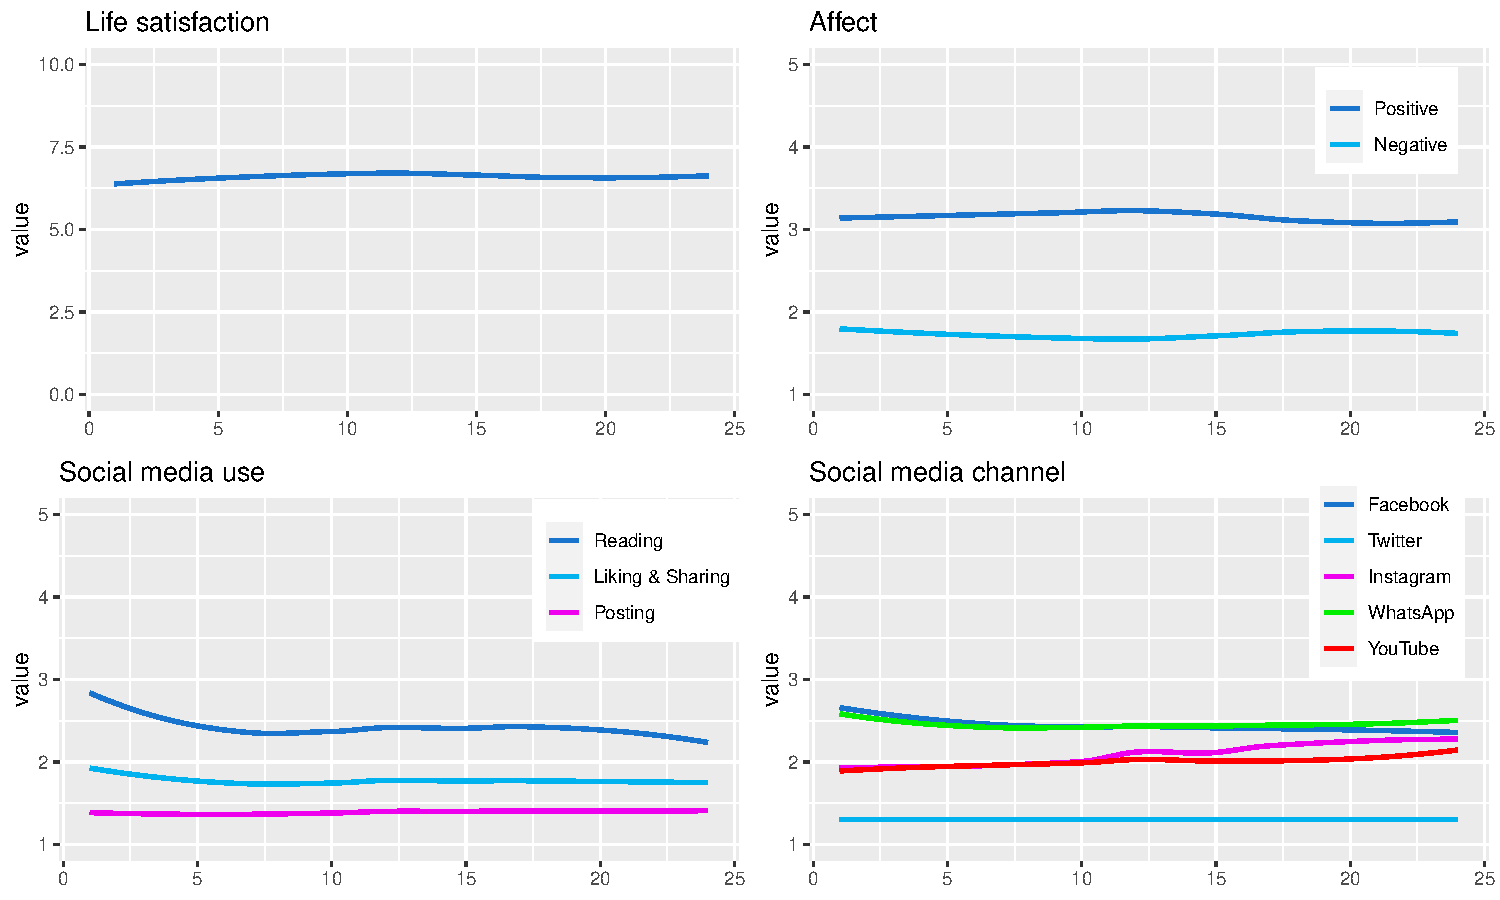
\includegraphics[width=\textwidth]{figures/fig_descriptives} \caption{Well-being and media use across the 32 waves. Note. Values obtained from mixed effect models, with participants and waves as grouping factors and without additional predictors.}\label{fig:fig-descriptives}
\end{figure}

Using the average values across all waves, which provides a stable picture of the general relations, I next looked at the correlations between social media use and well-being (see Figure \ref{fig:fig-correlations}).
Several interesting patterns emerged.
In general, people who spend more time engaging with COVID-19 related content on social media reported reduced well-being.
Users who spend more time reading, liking and sharing, and posting COVID-19 related content were less satisfied with their lives.
They also showed slightly less positive affect.
This overall negative picture was even more pronounced for negative affect.
People who engaged more with COVID-19 related content, including all types and channels of communication, reported substantially higher levels of negative affect.
For example, people who were more likely to post COVID-19 content had much higher levels of negative affect (\emph{r} = .56).
Note that these results represent between-person correlations, not causal within-person effects.

\begin{figure}
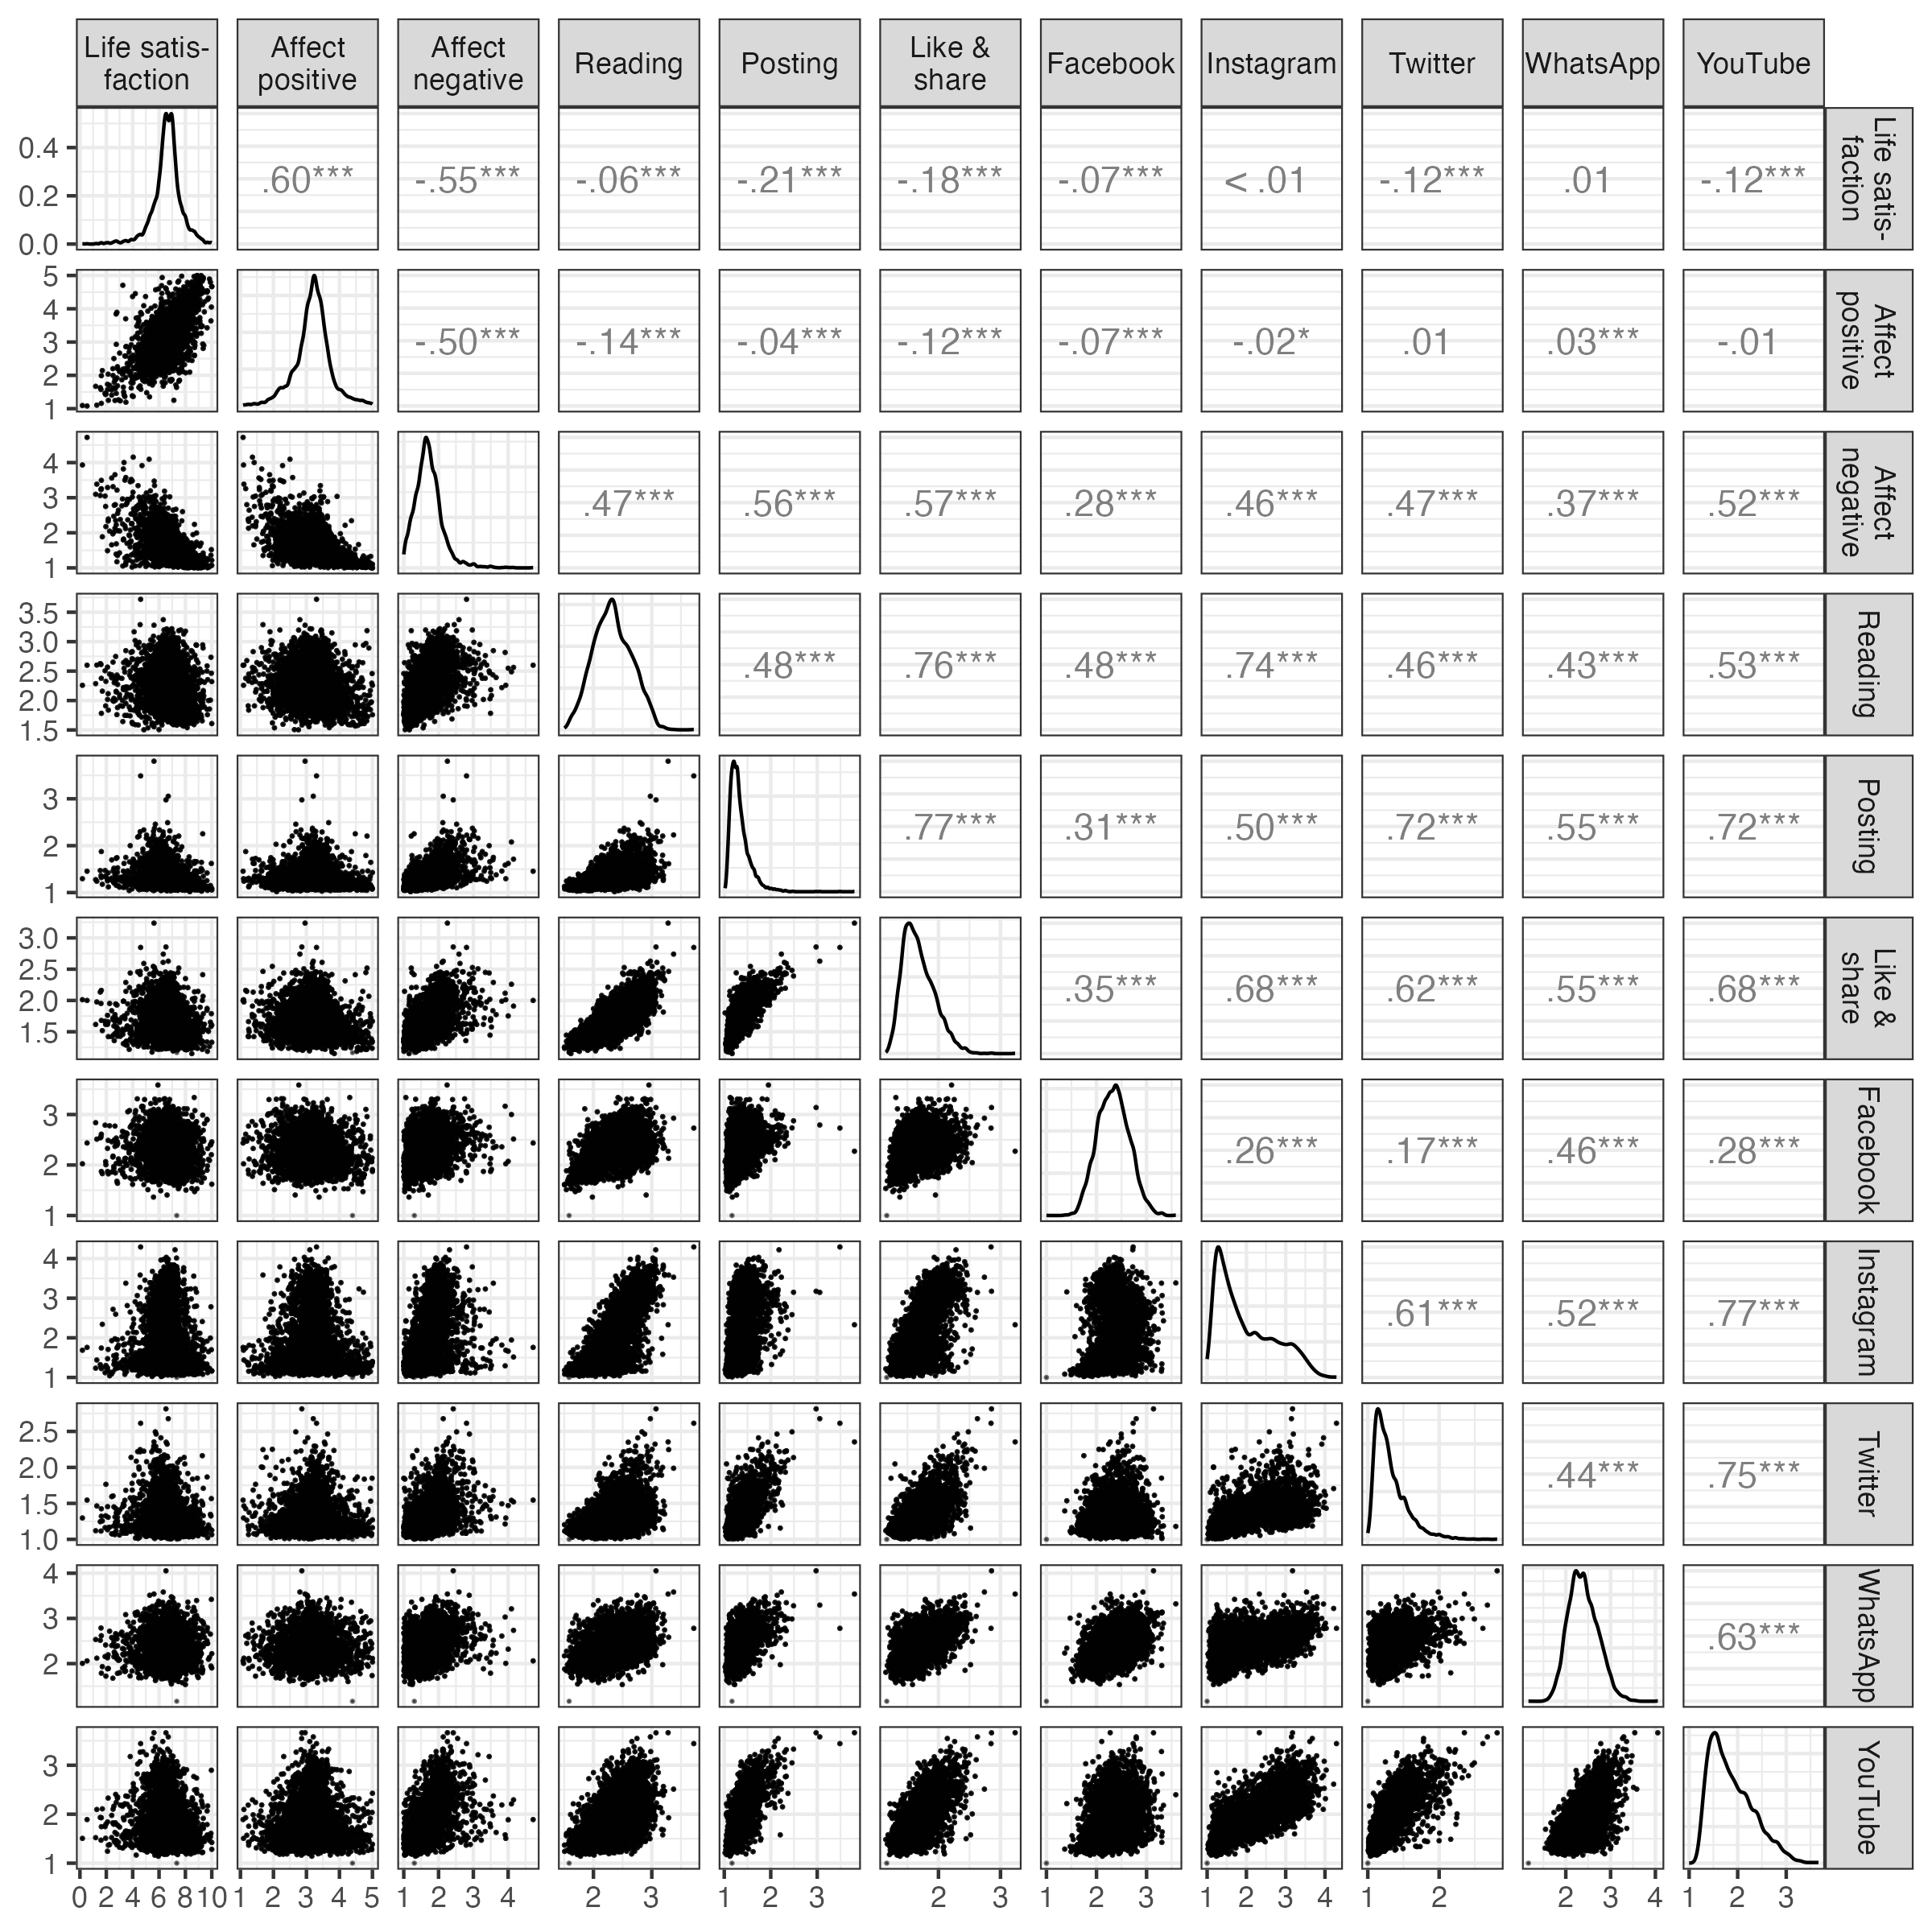
\includegraphics[width=\textwidth]{figures/fig_cor} \caption{Descriptives of the main variables, capturing well-being and social media use with their average values across all waves. Upper triangle: correlation coefficients; diagonal: density plots; lower triangle: scatter plots.}\label{fig:fig-correlations}
\end{figure}

\hypertarget{preregistered-analyses}{%
\subsection{Preregistered Analyses}\label{preregistered-analyses}}

\hypertarget{social-media-communication-types}{%
\subsubsection{Social media communication types}\label{social-media-communication-types}}

The study's main hypothesis was that the causal effects of all types and channels of social media use on all facets of well-being would be trivial.
Regarding the effects of different communication types (i.e., reading, sharing, of posting about COVID-19 related content), all within-person effects fell completely within the a-priori defined null region (see Figure \ref{fig:fig-within}).
For example, respondents who used social media more frequently than usual to like or share COVID-19 related content did not show a simultaneous change in life satisfaction (\emph{b} = -0.02 {[}95\% CI -0.08, 0.03{]}).
As a result, the hypothesis of trivial effects was supported for all COVID-19 related types of social media communication.

However, three effects stood out, as they were significantly different from zero.
Users who read more COVID-19 related content than usual reported slightly reduced levels of positive affect (\emph{b} = -0.03 {[}95\% CI -0.05, -0.01{]}).
Users who liked and shared more COVID-19 related content than usual also experienced slightly more negative affect than usual (\emph{b} = 0.05 {[}95\% CI 0.02, 0.08{]}).
Users who wrote more COVID-19 related posts than usual also experienced slightly more negative affect than usual (\emph{b} = 0.05 {[}95\% CI 0.02, 0.08{]}).

\hypertarget{social-media-communication-channels}{%
\subsubsection{Social media communication channels}\label{social-media-communication-channels}}

Regarding the COVID-19 related use of social media channels (i.e., Facebook, Instagram, WhatsApp, YouTube, and Twitter) the results were comparable (see Figure \ref{fig:fig-within}).
Changes in the frequency of using different social media channels to attain information regarding COVID-19 were unrelated to meaningful changes in well-being.
For example, respondents who used Facebook more frequently than usual to learn about COVID-19 did not show a simultaneous change in life satisfaction (\emph{b} \textless{} 0.01 {[}95\% CI -0.04, 0.04{]}).
In sum, the hypothesis of trivial effects was supported also for the COVID-19 related use of important social media channels.

That said, one effect differed substantially from zero.
Respondents who used Twitter more frequently than usual to attain COVID-19 related news reported slightly higher levels of negative affect than usual (\emph{b} = 0.01 {[}95\% CI \textless{} 0.01, 0.03{]}).
However, the effect was still completely inside of the null region, hence likely not large enough to be considered meaningful.

For an overview of all within-person effects, see Table \ref{tab:tab-within} and Figure \ref{fig:fig-within}.

\begin{figure}
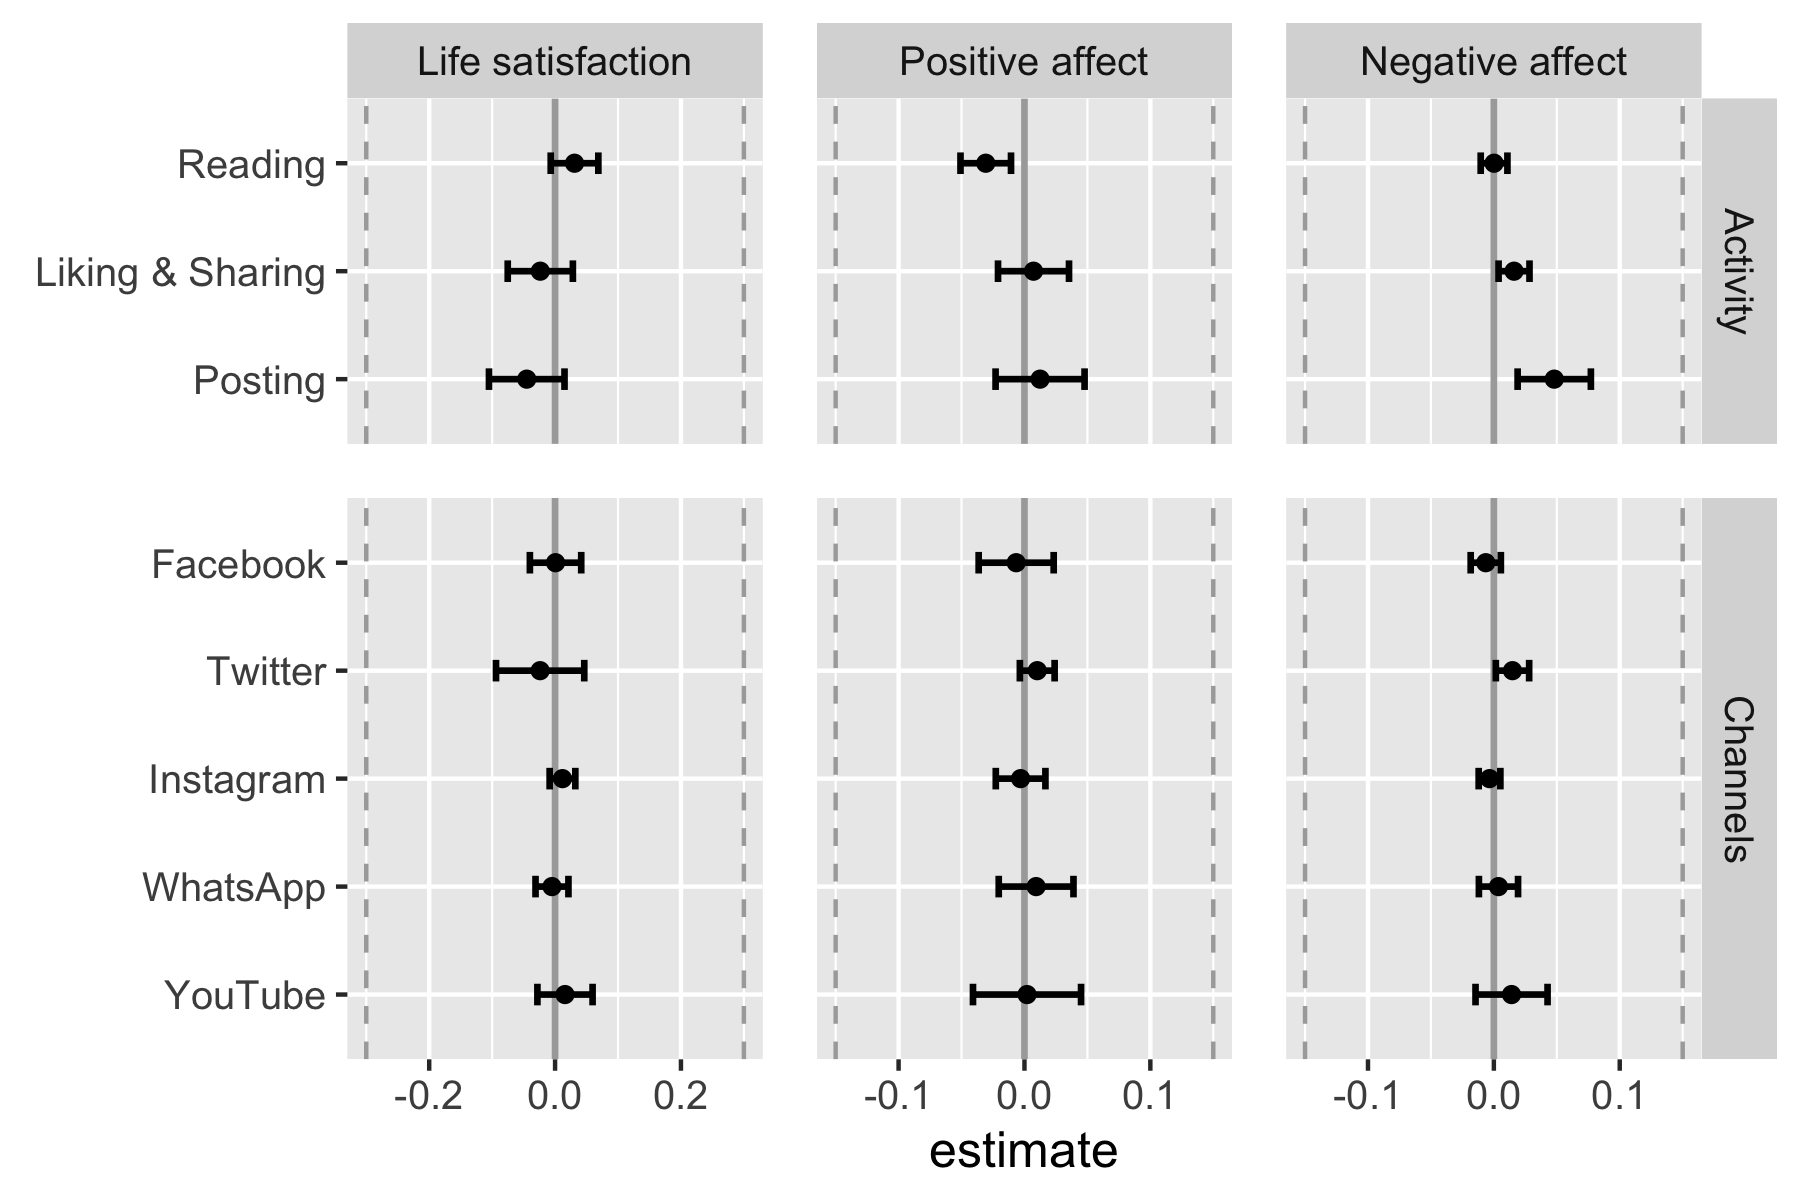
\includegraphics[width=\textwidth]{manuscript_files/figure-latex/fig-within-1} \caption{Within-person effects of COVID-19 related social media use on well-being. Note. The black estimates show the effects controlled for a large number of covariates (see text; preregistered); the grey estimates are without control variables (exploratory). The SESOI was b = |0.30| for life satisfaction and b = |0.15| for affect. Hence, all of the reported effects are not considered meaningful.}\label{fig:fig-within}
\end{figure}

\begin{table}[tbp]

\begin{center}
\begin{threeparttable}

\caption{\label{tab:tab-within}Overview of all within-person effects.}

\footnotesize{

\begin{tabular}{lrrrrr}
\toprule
 &  & \multicolumn{2}{c}{Confidence interval}  &  &\\
\cmidrule(r){3-4}
Predictor & \multicolumn{1}{c}{b} & \multicolumn{1}{c}{Lower} & \multicolumn{1}{c}{Higher} & \multicolumn{1}{c}{beta} & \multicolumn{1}{c}{p}\\
\midrule
Life satisfaction &  &  &  &  & \\
\ \ \ Reading & 0.03 & -0.01 & 0.07 & 0.02 & .091\\
\ \ \ Liking \& Sharing & -0.02 & -0.08 & 0.03 & -0.01 & .299\\
\ \ \ Posting & -0.05 & -0.11 & 0.01 & -0.02 & .114\\
\ \ \ Facebook & 0.00 & -0.04 & 0.04 & 0.00 & .964\\
\ \ \ Instagram & 0.01 & -0.01 & 0.03 & 0.01 & .226\\
\ \ \ WhatsApp & 0.00 & -0.03 & 0.02 & 0.00 & .664\\
\ \ \ YouTube & 0.02 & -0.03 & 0.06 & 0.01 & .402\\
\ \ \ Twitter & -0.02 & -0.09 & 0.05 & -0.01 & .420\\
Positive affect &  &  &  &  & \\
\ \ \ Reading & -0.03 & -0.05 & -0.01 & -0.04 & .011\\
\ \ \ Liking \& Sharing & 0.01 & -0.02 & 0.04 & 0.01 & .535\\
\ \ \ Posting & 0.01 & -0.02 & 0.05 & 0.01 & .404\\
\ \ \ Facebook & -0.01 & -0.04 & 0.02 & -0.01 & .581\\
\ \ \ Instagram & 0.00 & -0.02 & 0.02 & 0.00 & .704\\
\ \ \ WhatsApp & 0.01 & -0.02 & 0.04 & 0.01 & .444\\
\ \ \ YouTube & 0.00 & -0.04 & 0.04 & 0.00 & .904\\
\ \ \ Twitter & 0.01 & 0.00 & 0.02 & 0.01 & .129\\
Negative affect &  &  &  &  & \\
\ \ \ Reading & 0.00 & -0.01 & 0.01 & 0.00 & .971\\
\ \ \ Liking \& Sharing & 0.02 & 0.00 & 0.03 & 0.02 & .019\\
\ \ \ Posting & 0.05 & 0.02 & 0.08 & 0.04 & .009\\
\ \ \ Facebook & -0.01 & -0.02 & 0.01 & -0.01 & .226\\
\ \ \ Instagram & 0.00 & -0.01 & 0.01 & 0.00 & .371\\
\ \ \ WhatsApp & 0.00 & -0.01 & 0.02 & 0.01 & .562\\
\ \ \ YouTube & 0.01 & -0.01 & 0.04 & 0.02 & .250\\
\ \ \ Twitter & 0.01 & 0.00 & 0.03 & 0.01 & .034\\
\bottomrule
\end{tabular}

}

\end{threeparttable}
\end{center}

\end{table}

\hypertarget{exploratory-analyses}{%
\subsection{Exploratory Analyses}\label{exploratory-analyses}}

To contextualize the results reported above and to see if the study included any meaningful effects at all, I also looked at the effect sizes of the covariates.
Because each variable featured different response options, which would require defining a SESOI for each variable, I hence report the results of the standardized scales, which allows for a better comparison across the differently scaled variables.
Here, we can build on Cohen's convention that small effects begin at \emph{r} = \textbar.10\textbar.

The results showed that several effects crossed or fell completely outside of the SESOI.
They can hence be considered meaningful.
For example, if physical health decreased, this had a meaningful detrimental impact on life satisfaction (\(\beta\) = .18 {[}95\% CI .16, .20{]}), positive affect (\(\beta\) = .17 {[}95\% CI .16, .18{]}), and negative affect (\(\beta\) = -.18 {[}95\% CI -.19, -.17{]}).
Spending more time outside to exercise meaningfully increased positive affect (\(\beta\) = .12 {[}95\% CI .11, .13{]}).
Being more satisfied with the current democratic system meaningfully increased life satisfaction (\(\beta\) = .13 {[}95\% CI .12, .14{]}).
The strongest aspect affecting well-being was internal locus of control.
If people felt more in control of their lives, this strongly increased both life satisfaction (\(\beta\) = .31 {[}95\% CI .28, .34{]}) and
positive affect (\(\beta\) = .27 {[}95\% CI .25, .29{]}),
while decreasing negative affect (\(\beta\) = -.28 {[}95\% CI -.30, -.26{]}).

For an overview, see Figure \ref{fig:fig-control}.

\begin{figure}
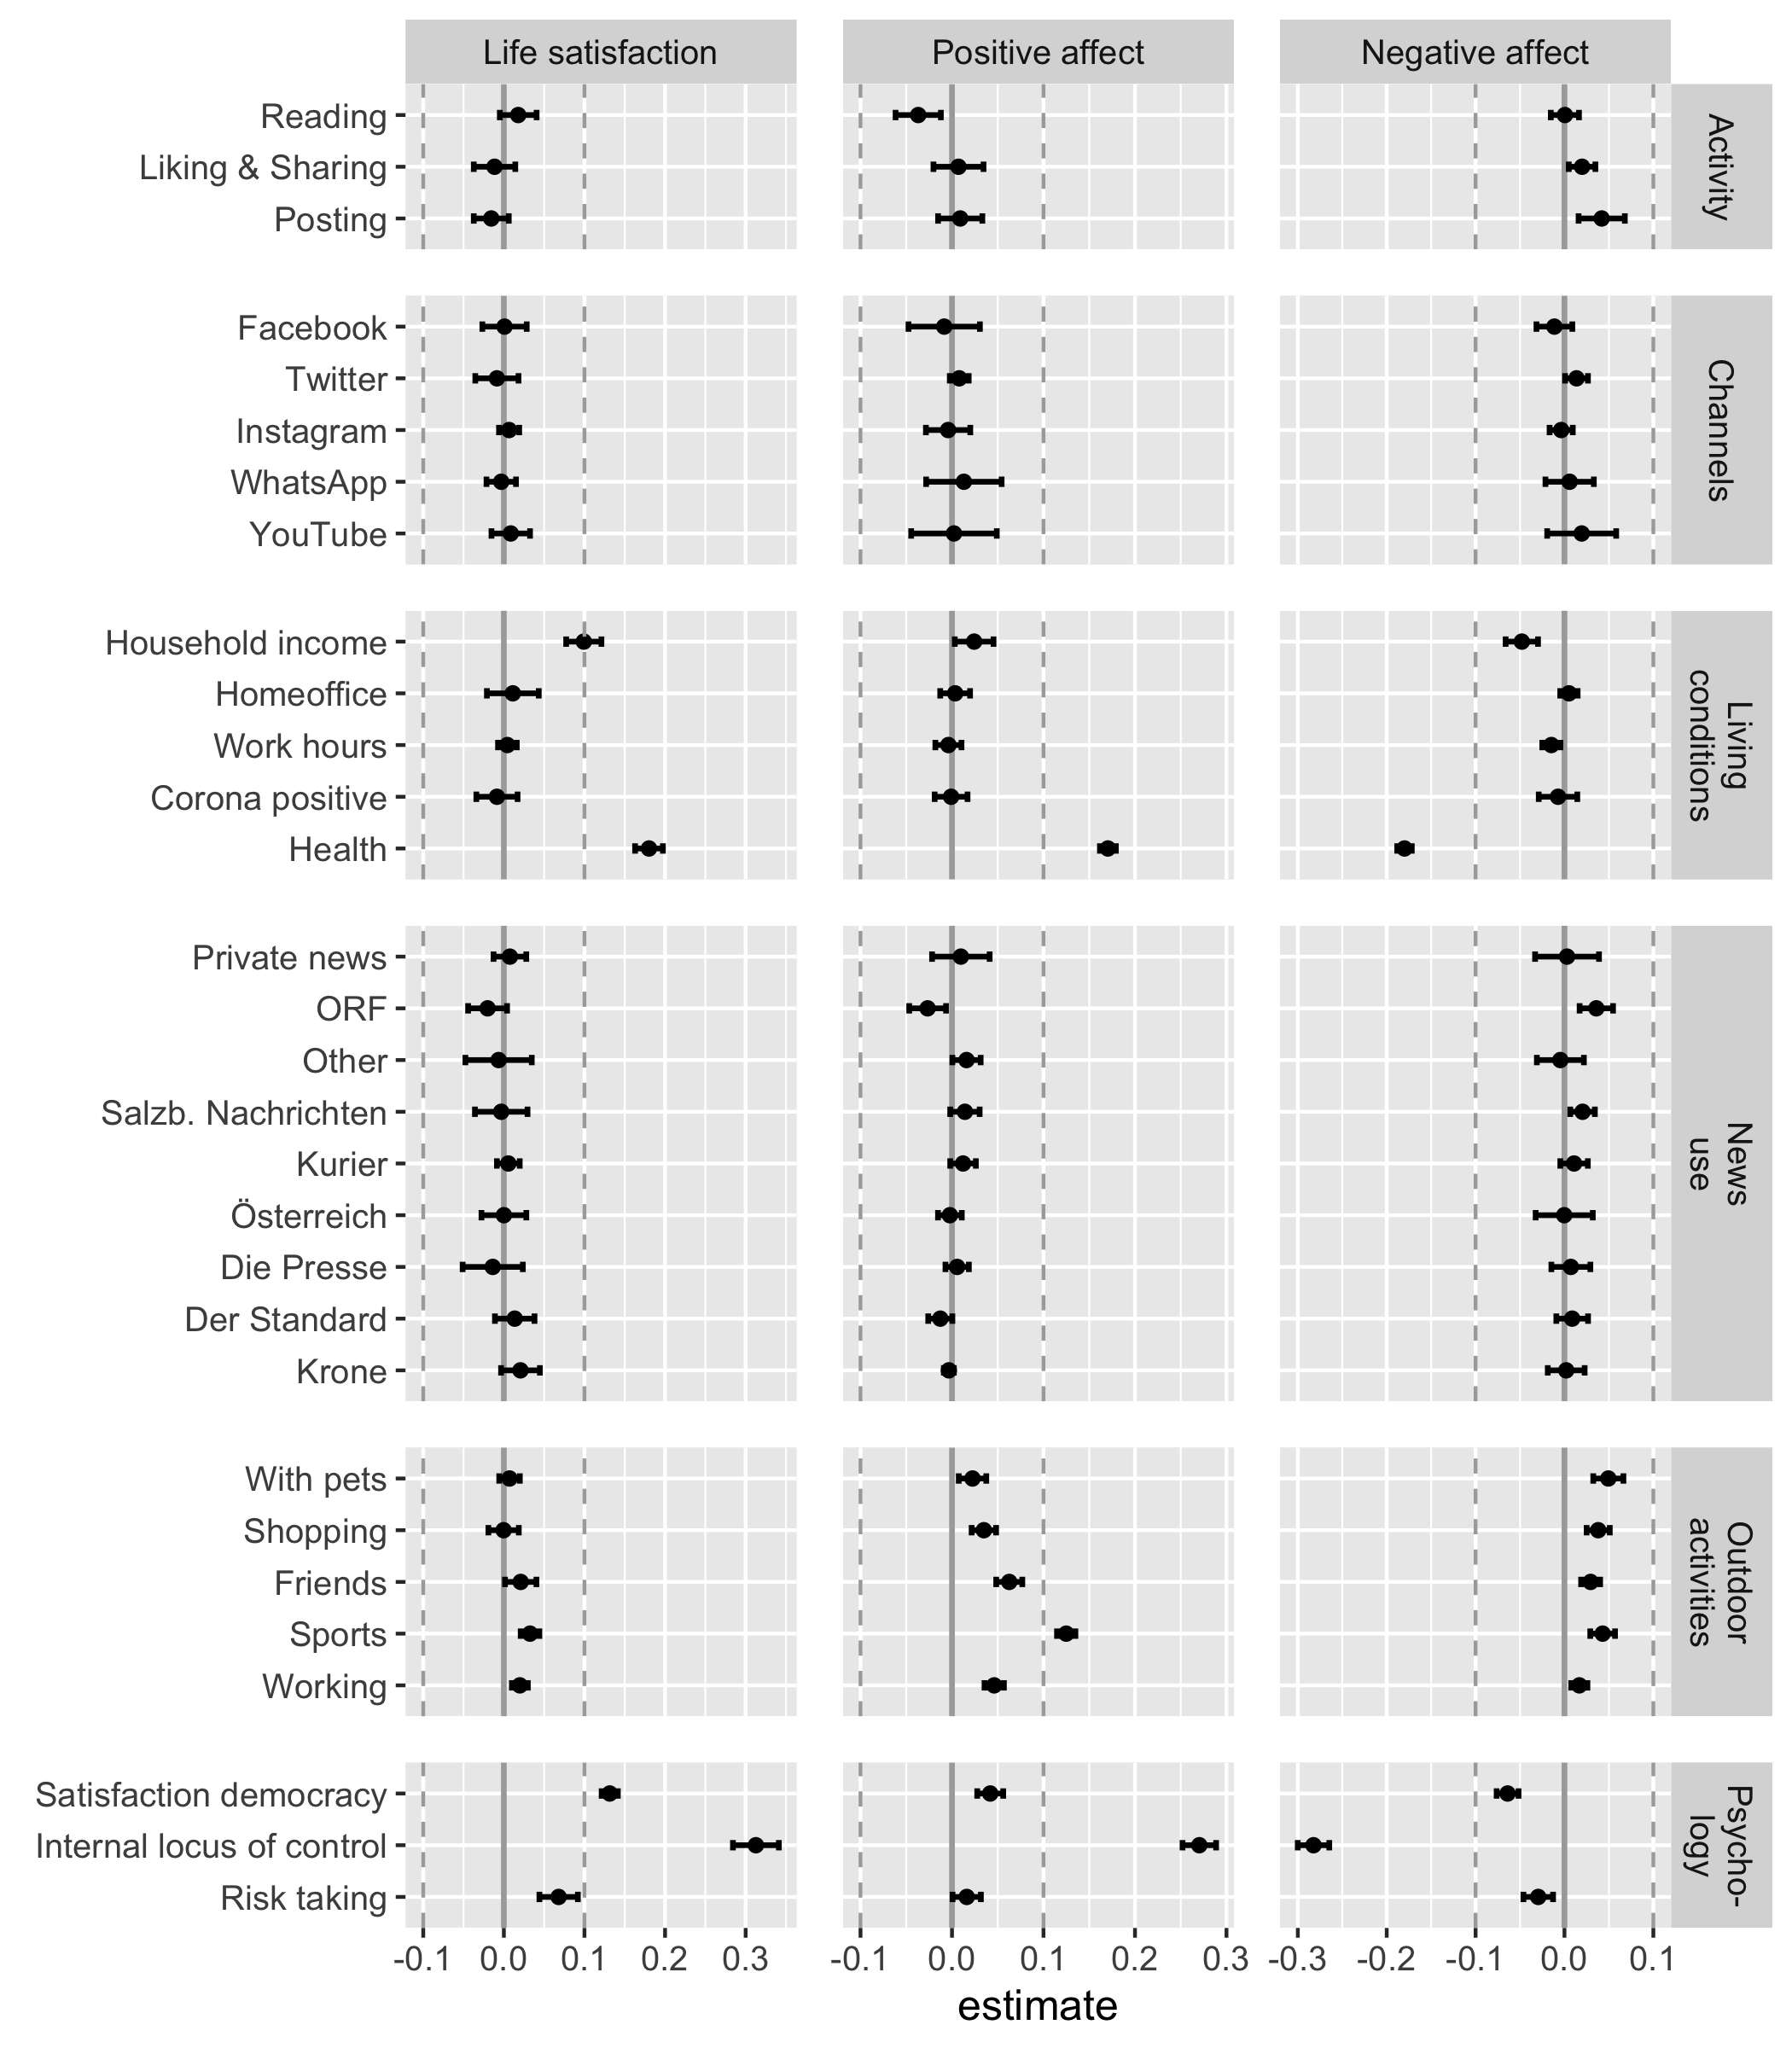
\includegraphics[width=\textwidth]{manuscript_files/figure-latex/fig-control-1} \caption{Results of main variables together with covariates to provide context. All variables standardized. SESOI: beta = |.10|}\label{fig:fig-control}
\end{figure}

\hypertarget{discussion}{%
\section{Discussion}\label{discussion}}

Based on a panel study with 32 waves largely representative of the Austrian population, this study analyzed the effects of COVID-19 related social media use on well-being.
Between person correlation analyses showed that more active users of COVID-19 related content on social media also reported decreased well-being.
The within-person relations, which are more informative regarding causal effects, showed a different pattern, however.
If people consumed more COVID-19 content on social media than usual, this did not meaningfully reduce their well-being.
Several statistically significant effects were found, but these were very small.
For example, people who liked and shared more COVID-19 related posts than usual reported slightly higher levels of negative affect.
Posting more content about COVID-19 than usual slightly increased negative affect.
People who read more COVID-19 related posts than usual reported slightly decreased positive affect.
Using Twitter for COVID-19 related content slightly increased negative affect.
Again, although all of these within-person effects were statistically significant, they were very small, smaller than the predefined smallest effect size of interest.
According to the preregistered procedure, they should hence be considered irrelevant.
Other factors, for which we would expect to find meaningful effects, such as health or sports, indeed showed substantial and meaningful impacts on well-being.
In conclusion, COVID-19 related activity on social media was not a particularly strong influence on peoples' well-being.
The results do not support the popular fears that ``doomscrolling'' or overusing social media during times of crises constitutes a relevant risk for well-being.

These specific observations notwithstanding, several general trends can be observed.
First, overall the results do suggest that effects of COVID-19 related social media use on well-being tend to take place in the negative as opposed to the positive spectrum.
Although very small, four statistically significant negative results of COVID-19 related social media use on well-being were found.
Not a single positive effect emerged.
Also note that in the analyses several control variables were included, ruling out plausible alternative explanations for the negative results.
For example, it was controlled for whether or not participants contracted a COVID-19 infection during a specific wave.
Hence, we can rule out the alternative explanation that having an infection was the root cause of increased communication and reduced well-being.

Second, significant outcomes emerged for positive or negative affect, but not for life satisfaction.
Life satisfaction was stable and not affected by any type or channel of social media communication.
The more fluctuating positive and negative affect, however, were affected.
Liking, sharing, and posting COVID-19 related content, and spending time on Twitter to browse COVID-19 related content, all negatively influenced affect.
This is aligned with prior findings which showed that social media can trigger negative affect but does not reduce life satisfaction (Huang, 2017).
Conversations about COVID-19 on social media are often extreme, negative, or aggressive (Fan et al., 2020).
More deeply engaging with this type of content could negatively affect active authors.
The hypothesis that tonality could explain the negative effects is especially supported by the observation that spending more time on Twitter than usual increased negative affect.
Communication on Twitter is often found to be more negative and impolite compared to other SNSs (Halpern \& Gibbs, 2013).
Consuming more negative and misleading information could hence explain the (slightly) increased levels of negative affect.

Third, the results show that it makes sense to analyze different communication types and communication channels.
Reading reduced positive affect, while liking, sharing and commenting increased negative affect.
Whereas it was often stated that passive use is bad and active use good (Verduyn et al., 2015), this pattern thus did not emerge here.
Instead, all three types were negative.
The results hence support the findings from Valkenburg et al. (2022), who also could not confirm the claim that active use is good and that passive use is bad.
Focusing on communication channels, Twitter seems to be more negative, as has often been observed (Halpern \& Gibbs, 2013).
But, again, all of these effects are very small.
Future research might elaborate on these specific relations to probe their stability and relevance.

Taken together, the results are hence aligned with the underlying theoretical models and prior empirical results.
The findings support the Different Susceptibility to Media Effects Theory, which states that effects are generally small and depend on the type of communication.
The results are well-aligned with mood management theory (Zillmann, 1988) or the uses and gratifications approach (Katz et al., 1973), whose premises preclude particularly negative effects of routine and widespread media consumption.
If the effects of social media were indeed profoundly negative on average, then people likely would not spend so much time on social media engaging with COVID-19 content.
Likewise, recent empirical studies and meta-analyses reported rather small negative effects, too.
Several studies found that the effects of various types of social media use on well-being are small, often too small to matter (Bendau et al., 2021; Ferguson et al., 2021; Meier \& Reinecke, 2020; Orben, 2020), echoing the results obtained here.

In light of the overall very small effects, engaging in COVID 19-related social media use should not be a major concern for one's well-being.
That said, the results still imply that it does make sense to critically reflect upon COVID-19 related social media use.
On average, it is likely more beneficial to post less actively about COVID-19 on social media and to spend less time on Twitter consuming COVID-19 related content.
The results allow us to reject a positive effect: Writing more posts on social media will likely not increase well-being.

\hypertarget{limitations}{%
\subsection{Limitations}\label{limitations}}

Focusing on within-person effects and controlling for several potential confounders, this study provides an improved perspective on assessing causality.
However, three major challenges remain.
First, it could be that the timing of the interval was wrong; it could be that effects unfold in shorter or longer intervals.
Next, it could be that there was not sufficient variance in media use and well-being.
Without sufficient variability, statistical models cannot detect existing effects.
Third, it is necessary to control for \emph{all} relevant confounding third variables.
Although this study included are large list of confounders, it could still be that crucial variables were missed (Zillmann, 1988).
To borrow the words from Rohrer and Murayama (2021), there is no such thing as ``the'' effect of social media use on well-being.
The results reported here are hence contingent on the design I used.
To document how effects unfold, future research needs to employ different study designs probing different intervals.
More thought needs to be invested in what factors to control for, and I hope this study provides a first step into this direction.

Although I had already reduced the predefined SESOIs to be less conservative, one could argue they were still too large.
Media use is only one aspect of several factors that simultaneously affect well-being.
Is it realistic to expect that changing only \emph{one} of these aspects should already manifest in a detectable change in well-being?
Or would it make more sense to expect that thoroughly committing to say \emph{two} activities (e.g.~regularly exercising \emph{and} establishing a reading habit) should then cause a detectable improvement in well-being?
Practically, this would imply a SESOI half the size defined here, namely \emph{b} = \textbar.15\textbar{} for life satisfaction and \emph{b} = \textbar.075\textbar{} for affect.
In the case of this study, however, even halving the SESOI would not make a difference.
All but one effect would still be completely in the null region, and no effect would fall completely outside of the null region.
I encourage future research to elaborate on what effect sizes are considered meaningful and what not.

Both media use and well-being were measured using self-reports.
Because assessing well-being necessarily requires introspection, using self-reports for affect and life satisfaction is adequate.
However, for social media use objective measures are clearly preferable, as people often cannot reliably estimate their use (Scharkow, 2016).
At the same time, most objective measures cannot capture the content or the motivation of use.
Hence, for the type of research question analyzed here, it still seems necessary to use self-reported measures.
In many cases they can still be informative (Verbeij et al., 2021).

Being collected in a single country, the generalizability of the results is limited.
The results apply primarily to the more Western sphere.
They might not hold true in other cultures, especially cultures with a different media landscape or alternative social media channels.

\hypertarget{conclusion}{%
\subsection{Conclusion}\label{conclusion}}

In this study, COVID-19 related social media use did not meaningfully affect well-being.
Very small negative effects were found for writing COVID-19 related posts, sharing COVID-19 related content, and spending more time than usual on Twitter.
Factors other than social media use, however, were meaningfully related to well-being, including physical health, exercise, satisfaction with democracy, or believing that one is in control of one's life.
Hence, when trying to improve well-being during a pandemic, instead of focusing on social media it seems more fruitful to address other, more pertinent societal problems related to health care, regular exercise, or a functioning democratic system.

\newpage

\hypertarget{references}{%
\section{References}\label{references}}

\hypertarget{refs}{}
\begin{CSLReferences}{1}{0}
\leavevmode\vadjust pre{\hypertarget{ref-bellFixedRandomEffects2019}{}}%
Bell, A., Fairbrother, M., \& Jones, K. (2019). Fixed and random effects models: Making an informed choice. \emph{Quality \& Quantity}, \emph{53}(2), 1051--1074. \url{https://doi.org/10.1007/s11135-018-0802-x}

\leavevmode\vadjust pre{\hypertarget{ref-bendauAssociationsCOVID19Related2021}{}}%
Bendau, A., Petzold, M. B., Pyrkosch, L., Mascarell Maricic, L., Betzler, F., Rogoll, J., Große, J., Ströhle, A., \& Plag, J. (2021). Associations between {COVID-19} related media consumption and symptoms of anxiety, depression and {COVID-19} related fear in the general population in {Germany}. \emph{European Archives of Psychiatry and Clinical Neuroscience}, \emph{271}(2), 283--291. \url{https://doi.org/10.1007/s00406-020-01171-6}

\leavevmode\vadjust pre{\hypertarget{ref-beyensSocialMediaUse2021}{}}%
Beyens, I., Pouwels, J. L., van Driel, I. I., Keijsers, L., \& Valkenburg, P. M. (2021). Social media use and adolescents' well-being: {Developing} a typology of person-specific effect patterns. \emph{Communication Research}. \url{https://doi.org/10.1177/00936502211038196}

\leavevmode\vadjust pre{\hypertarget{ref-bradleyStressMoodSmartphone2021}{}}%
Bradley, A., \& Howard, A. (2021). \emph{Stress, mood, and smartphone use in {University} students: {A} 12-week longitudinal study}. \url{https://doi.org/10.31219/osf.io/frvpb}

\leavevmode\vadjust pre{\hypertarget{ref-buchiDigitalWellbeingTheory2021}{}}%
Büchi, M. (2021). Digital well-being theory and research. \emph{New Media \& Society}, 146144482110568. \url{https://doi.org/10.1177/14614448211056851}

\leavevmode\vadjust pre{\hypertarget{ref-choiMediatedCommunicationMatters2021}{}}%
Choi, M., \& Choung, H. (2021). Mediated communication matters during the {COVID-19} pandemic: {The} use of interpersonal and masspersonal media and psychological well-being. \emph{Journal of Social and Personal Relationships}, \emph{38}(8), 2397--2418. \url{https://doi.org/10.1177/02654075211029378}

\leavevmode\vadjust pre{\hypertarget{ref-dienerAdvancesOpenQuestions2018}{}}%
Diener, E., Lucas, R. E., \& Oishi, S. (2018). Advances and open questions in the science of subjective well-being. \emph{Collabra: Psychology}, \emph{4}(1), 15. \url{https://doi.org/10.1525/collabra.115}

\leavevmode\vadjust pre{\hypertarget{ref-dienesUsingBayesGet2014}{}}%
Dienes, Z. (2014). Using {Bayes} to get the most out of non-significant results. \emph{Frontiers in Psychology}, \emph{5}. \url{https://doi.org/10.3389/fpsyg.2014.00781}

\leavevmode\vadjust pre{\hypertarget{ref-dienlinImpactDigitalTechnology2020}{}}%
Dienlin, T., \& Johannes, N. (2020). The impact of digital technology use on adolescent well-being. \emph{Dialogues in Clinical Neuroscience}, \emph{22}(2), 135--142. \url{https://doi.org/doi:10.31887/DCNS.2020.22.2/tdienlin}

\leavevmode\vadjust pre{\hypertarget{ref-dienlinDisplacementReinforcementReciprocity2017}{}}%
Dienlin, T., Masur, P. K., \& Trepte, S. (2017). Displacement or reinforcement? {The} reciprocity of {FtF}, {IM}, and {SNS} communication and their effects on loneliness and life satisfaction. \emph{Journal of Computer-Mediated Communication}, \emph{22}(2), 71--87. \url{https://doi.org/10.1111/jcc4.12183}

\leavevmode\vadjust pre{\hypertarget{ref-dormannOptimalTimeLags2015}{}}%
Dormann, C., \& Griffin, M. A. (2015). Optimal time lags in panel studies. \emph{Psychological Methods}, \emph{20}(4), 489--505. \url{https://doi.org/10.1037/met0000041}

\leavevmode\vadjust pre{\hypertarget{ref-dornemannHowGoodBad2021}{}}%
Dörnemann, A., Boenisch, N., Schommer, L., Winkelhorst, L., \& Wingen, T. (2021). \emph{How do good and bad news impact mood during the {Covid-19} pandemic? {The} role of similarity}. \url{https://doi.org/10.31219/osf.io/sy2kd}

\leavevmode\vadjust pre{\hypertarget{ref-edenMediaCopingCOVID192020}{}}%
Eden, A. L., Johnson, B. K., Reinecke, L., \& Grady, S. M. (2020). Media for coping during {COVID-19} social distancing: {Stress}, anxiety, and psychological well-being. \emph{Frontiers in Psychology}, \emph{11}, 577639. \url{https://doi.org/10.3389/fpsyg.2020.577639}

\leavevmode\vadjust pre{\hypertarget{ref-europeansocialsurveyESS9Edition20182021}{}}%
European Social Survey. (2021). \emph{{ESS9} edition 3.1 - 2018 {Documentation Report}}. \url{https://www.europeansocialsurvey.org/docs/round9/survey/ESS9_data_documentation_report_e03_1.pdf}

\leavevmode\vadjust pre{\hypertarget{ref-fanStigmatizationSocialMedia2020}{}}%
Fan, L., Yu, H., \& Yin, Z. (2020). Stigmatization in social media: {Documenting} and analyzing hate speech for {\textsc{COVID}} ‐19 on {Twitter}. \emph{Proceedings of the Association for Information Science and Technology}, \emph{57}(1). \url{https://doi.org/10.1002/pra2.313}

\leavevmode\vadjust pre{\hypertarget{ref-fergusonThisMetaanalysisScreen2021}{}}%
Ferguson, C. J., Kaye, L. K., Branley-Bell, D., Markey, P., Ivory, J. D., Klisanin, D., Elson, M., Smyth, M., Hogg, J. L., McDonnell, D., Nichols, D., Siddiqui, S., Gregerson, M., \& Wilson, J. (2021). Like this meta-analysis: {Screen} media and mental health. \emph{Professional Psychology: Research and Practice}. \url{https://doi.org/10.1037/pro0000426}

\leavevmode\vadjust pre{\hypertarget{ref-funderEvaluatingEffectSize2019}{}}%
Funder, D. C., \& Ozer, D. J. (2019). Evaluating effect size in psychological research: {Sense} and nonsense. \emph{Advances in Methods and Practices in Psychological Science}, \emph{2}(2), 156--168. \url{https://doi.org/10.1177/2515245919847202}

\leavevmode\vadjust pre{\hypertarget{ref-guazziniSecondWaveAnalysis2022}{}}%
Guazzini, A., Pesce, A., Marotta, L., \& Duradoni, M. (2022). Through the second wave: {Analysis} of the psychological and perceptive changes in the {Italian} population during the {COVID-19} pandemic. \emph{International Journal of Environmental Research and Public Health}, \emph{19}(3), 1635. \url{https://doi.org/10.3390/ijerph19031635}

\leavevmode\vadjust pre{\hypertarget{ref-halpernSocialMediaCatalyst2013}{}}%
Halpern, D., \& Gibbs, J. (2013). Social media as a catalyst for online deliberation? {Exploring} the affordances of {Facebook} and {YouTube} for political expression. \emph{Computers in Human Behavior}, \emph{29}(3), 1159--1168. \url{https://doi.org/10.1016/j.chb.2012.10.008}

\leavevmode\vadjust pre{\hypertarget{ref-hamakerWhyResearchersShould2014}{}}%
Hamaker, E. L. (2014). Why researchers should think "within-person": {A} paradigmatic rationale. In M. R. Mehl, T. S. Conner, \& M. Csikszentmihalyi (Eds.), \emph{Handbook of research methods for studying daily life} (Paperback ed.). {Guilford}.

\leavevmode\vadjust pre{\hypertarget{ref-huangTimeSpentSocial2017}{}}%
Huang, C. (2017). Time spent on social network sites and psychological well-being: {A} meta-analysis. \emph{Cyberpsychology, Behavior and Social Networking}, \emph{20}(6), 346--354. \url{https://doi.org/10.1089/cyber.2016.0758}

\leavevmode\vadjust pre{\hypertarget{ref-katzUsesGratificationsResearch1973}{}}%
Katz, E., Blumler, J. G., \& Gurevitch, M. (1973). Uses and {Gratifications Research}. \emph{Public Opinion Quarterly}, \emph{37}(4), 509. \url{https://doi.org/10.1086/268109}

\leavevmode\vadjust pre{\hypertarget{ref-kittelAustrianCoronaPanel2021}{}}%
Kittel, B., Kritzinger, S., Boomgaarden, H., Prainsack, B., Eberl, J.-M., Kalleitner, F., Lebernegg, N. S., Partheymüller, J., Plescia, C., Schiestl, D. W., \& Schlogl, L. (2021). The {Austrian Corona Panel Project}: Monitoring individual and societal dynamics amidst the {COVID-19} crisis. \emph{European Political Science}, \emph{20}(2), 318--344. \url{https://doi.org/10.1057/s41304-020-00294-7}

\leavevmode\vadjust pre{\hypertarget{ref-kittelAustrianCoronaPanel2020}{}}%
Kittel, B., Kritzinger, S., Boomgaarden, H., Prainsack, B., Eberl, J.-M., Kalleitner, F., Lebernegg, N. S., Partheymüller, J., Plescia, C., Schiestl, D. W., \& Schlogl, L. (2020). \emph{Austrian {Corona Panel Project} ({SUF} edition)} {[}Data set{]}. {AUSSDA}. \url{https://doi.org/10.11587/28KQNS}

\leavevmode\vadjust pre{\hypertarget{ref-kleinDarklySoothingCompulsion2021}{}}%
Klein, J. (2021, March 3). \emph{The darkly soothing compulsion of 'doomscrolling'}. \url{https://www.bbc.com/worklife/article/20210226-the-darkly-soothing-compulsion-of-doomscrolling}

\leavevmode\vadjust pre{\hypertarget{ref-latikkaLonelinessPsychologicalDistress2022}{}}%
Latikka, R., Koivula, A., Oksa, R., Savela, N., \& Oksanen, A. (2022). Loneliness and psychological distress before and during the {COVID-19} pandemic: {Relationships} with social media identity bubbles. \emph{Social Science \& Medicine}, \emph{293}, 114674. \url{https://doi.org/10.1016/j.socscimed.2021.114674}

\leavevmode\vadjust pre{\hypertarget{ref-liuRelationOfficialWhatsAppdistributed2020}{}}%
Liu, J. C. J., \& Tong, E. M. W. (2020). The relation between official {WhatsApp-distributed COVID-19} news exposure and psychological symptoms: Cross-sectional survey study. \emph{Journal of Medical Internet Research}, \emph{22}(9), e22142. \url{https://doi.org/10.2196/22142}

\leavevmode\vadjust pre{\hypertarget{ref-lucasAdaptationSetpointModel2007}{}}%
Lucas, R. E. (2007). Adaptation and the set-point model of subjective well-being. \emph{Current Directions in Psychological Science}, \emph{16}(2), 75--79. \url{https://doi.org/10.1111/j.1467-8721.2007.00479.x}

\leavevmode\vadjust pre{\hypertarget{ref-lucasWhyCrossLaggedPanel2022}{}}%
Lucas, R. E. (2022). \emph{Why the {Cross-Lagged Panel Model} is {Almost Never} the {Right Choice}} {[}Preprint{]}. {PsyArXiv}. \url{https://doi.org/10.31234/osf.io/pkec7}

\leavevmode\vadjust pre{\hypertarget{ref-lykkenHappinessWhatStudies1999}{}}%
Lykken, D. T. (1999). \emph{Happiness: {What} studies on twins show us about nature, nurture, and the happiness set-point}. {Golden Books}.

\leavevmode\vadjust pre{\hypertarget{ref-marcianoDynamicsAdolescentsSmartphone2022}{}}%
Marciano, L., Driver, C. C., Schulz, P. J., \& Camerini, A.-L. (2022). Dynamics of adolescents' smartphone use and well-being are positive but ephemeral. \emph{Scientific Reports}, \emph{12}(1), 1316. \url{https://doi.org/10.1038/s41598-022-05291-y}

\leavevmode\vadjust pre{\hypertarget{ref-meierDoesPassiveSocial2022}{}}%
Meier, A., \& Krause, H.-V. (2022). \emph{Does passive social media use harm well-being? {An} adversarial review} {[}Preprint{]}. {PsyArXiv}. \url{https://doi.org/10.31234/osf.io/nvbwh}

\leavevmode\vadjust pre{\hypertarget{ref-meierComputermediatedCommunicationSocial2020a}{}}%
Meier, A., \& Reinecke, L. (2020). Computer-mediated communication, social media, and mental health: {A} conceptual and empirical meta-review. \emph{Communication Research}, 009365022095822. \url{https://doi.org/10.1177/0093650220958224}

\leavevmode\vadjust pre{\hypertarget{ref-normanInterpretationChangesHealthrelated2003}{}}%
Norman, G., Sloan, J., \& Wyrwich, K. (2003). Interpretation of changes in health-related quality of life: {The} remarkable universality of half a standard deviation. \emph{Medical Care}, \emph{41}(5), 582--592. \href{Retrieved\%20from\%20http://www.jstor.org/stable/3768017}{Retrieved from http://www.jstor.org/stable/3768017}

\leavevmode\vadjust pre{\hypertarget{ref-orbenTeenagersScreensSocial2020}{}}%
Orben, A. (2020). Teenagers, screens and social media: A narrative review of reviews and key studies. \emph{Social Psychiatry and Psychiatric Epidemiology}, \emph{55}(4), 407--414. \url{https://doi.org/10.1007/s00127-019-01825-4}

\leavevmode\vadjust pre{\hypertarget{ref-pelletierOneSizeDoesn2020}{}}%
Pelletier, M. J., Krallman, A., Adams, F. G., \& Hancock, T. (2020). One size doesn't fit all: A uses and gratifications analysis of social media platforms. \emph{Journal of Research in Interactive Marketing}, \emph{14}(2), 269--284. \url{https://doi.org/10.1108/JRIM-10-2019-0159}

\leavevmode\vadjust pre{\hypertarget{ref-riehmAssociationsMediaExposure2020}{}}%
Riehm, K. E., Holingue, C., Kalb, L. G., Bennett, D., Kapteyn, A., Jiang, Q., Veldhuis, C. B., Johnson, R. M., Fallin, M. D., Kreuter, F., Stuart, E. A., \& Thrul, J. (2020). Associations between media exposure and mental distress among {U}.{S}. Adults at the beginning of the {COVID-19} pandemic. \emph{American Journal of Preventive Medicine}, \emph{59}(5), 630--638. \url{https://doi.org/10.1016/j.amepre.2020.06.008}

\leavevmode\vadjust pre{\hypertarget{ref-rohrerThinkingClearlyCorrelations2018}{}}%
Rohrer, J. M. (2018). Thinking clearly about correlations and causation: {Graphical} causal models for observational data. \emph{Advances in Methods and Practices in Psychological Science}, \emph{24}(2), 251524591774562. \url{https://doi.org/10.1177/2515245917745629}

\leavevmode\vadjust pre{\hypertarget{ref-rohrerTheseAreNot2021}{}}%
Rohrer, J. M., \& Murayama, K. (2021). \emph{These are not the effects you are looking for: {Causality} and the within-/between-person distinction in longitudinal data analysis}. {PsyArXiv}. \url{https://doi.org/10.31234/osf.io/tg4vj}

\leavevmode\vadjust pre{\hypertarget{ref-sandstromDoomscrollingCOVIDNews2021}{}}%
Sandstrom, G., Buchanan, K., Aknin, L., \& Lotun, S. (2021, October 22). \emph{Doomscrolling {COVID} news takes an emotional toll -- here's how to make your social media a happier place}. {The Conversation}. \url{http://theconversation.com/doomscrolling-covid-news-takes-an-emotional-toll-heres-how-to-make-your-social-media-a-happier-place-170342}

\leavevmode\vadjust pre{\hypertarget{ref-scharkowAccuracySelfreportedInternet2016}{}}%
Scharkow, M. (2016). The accuracy of self-reported {Internet} use---{A} validation study using client log data. \emph{Communication Methods and Measures}, \emph{10}(1), 13--27. \url{https://doi.org/10.1080/19312458.2015.1118446}

\leavevmode\vadjust pre{\hypertarget{ref-sewallObjectivelyMeasuredDigital2021}{}}%
Sewall, C. J. R., Goldstein, T. R., \& Rosen, D. (2021). Objectively measured digital technology use during the {COVID-19} pandemic: {Impact} on depression, anxiety, and suicidal ideation among young adults. \emph{Journal of Affective Disorders}, \emph{288}, 145--147. \url{https://doi.org/10.1016/j.jad.2021.04.008}

\leavevmode\vadjust pre{\hypertarget{ref-sheldonStabilityHappinessTheories2014}{}}%
Sheldon, K. M., \& Lucas, R. E. (2014). \emph{Stability of happiness: Theories and evidence on whether happiness can change}. \url{http://site.ebrary.com/id/10891875}

\leavevmode\vadjust pre{\hypertarget{ref-stainbackCOVID1924News2020}{}}%
Stainback, K., Hearne, B. N., \& Trieu, M. M. (2020). {COVID-19} and the 24/7 {News Cycle}: {Does COVID-19 News Exposure Affect Mental Health}? \emph{Socius}, \emph{6}, 2378023120969339. \url{https://doi.org/10.1177/2378023120969339}

\leavevmode\vadjust pre{\hypertarget{ref-statistaAverageDailyTime2021}{}}%
Statista. (2021, May 21). \emph{Average daily time spent on social networks by users in the {United States} from 2018 to 2022}. \url{https://www.statista.com/statistics/1018324/us-users-daily-social-media-minutes/}

\leavevmode\vadjust pre{\hypertarget{ref-valkenburgDifferentialSusceptibilityMedia2013}{}}%
Valkenburg, P. M., \& Peter, J. (2013). The differential susceptibility to media effects model. \emph{Journal of Communication}, \emph{63}(2), 221--243. \url{https://doi.org/10.1111/jcom.12024}

\leavevmode\vadjust pre{\hypertarget{ref-valkenburgAssociationsActivePassive2022}{}}%
Valkenburg, P. M., van Driel, I. I., \& Beyens, I. (2022). The associations of active and passive social media use with well-being: {A} critical scoping review. \emph{New Media \& Society}, \emph{24}(2), 530--549. \url{https://doi.org/10.1177/14614448211065425}

\leavevmode\vadjust pre{\hypertarget{ref-verbeijSelfreportedMeasuresSocial2021}{}}%
Verbeij, T., Pouwels, J. L., Beyens, I., \& Valkenburg, P. M. (2021). \emph{Self-reported measures of social media use show high predictive validity} {[}Preprint{]}. {PsyArXiv}. \url{https://doi.org/10.31234/osf.io/c9bj7}

\leavevmode\vadjust pre{\hypertarget{ref-verduynPassiveFacebookUsage2015}{}}%
Verduyn, P., Lee, D. S., Park, J., Shablack, H., Orvell, A., Bayer, J., Ybarra, O., Jonides, J., \& Kross, E. (2015). Passive {Facebook} usage undermines affective well-being: {Experimental} and longitudinal evidence. \emph{Journal of Experimental Psychology: General}, \emph{144}(2), 480--488. \url{https://doi.org/10.1037/xge0000057}

\leavevmode\vadjust pre{\hypertarget{ref-wagnerAUTNESOnlinePanel2018}{}}%
Wagner, M., Aichholzer, J., Eberl, J.-M., Meyer, T. M., Berk, N., Büttner, N., Boomgaarden, H., Kritzinger, S., \& Müller, W. C. (2018). \emph{{AUTNES Online Panel Study} 2017 ({SUF} edition)} {[}Data set{]}. {AUSSDA}. \url{https://doi.org/10.11587/I7QIYJ}

\leavevmode\vadjust pre{\hypertarget{ref-worldhealthorganizationWellbeingMeasuresPrimary1998}{}}%
World Health Organization. (1998). \emph{Wellbeing measures in primary health care/{The Depcare Project}}.

\leavevmode\vadjust pre{\hypertarget{ref-yuePassiveSocialMedia2022}{}}%
Yue, Z., Zhang, R., \& Xiao, J. (2022). Passive social media use and psychological well-being during the {COVID-19} pandemic: {The} role of social comparison and emotion regulation. \emph{Computers in Human Behavior}, \emph{127}, 107050. \url{https://doi.org/10.1016/j.chb.2021.107050}

\leavevmode\vadjust pre{\hypertarget{ref-zillmannMoodManagementCommunication1988}{}}%
Zillmann, D. (1988). Mood {Management Through Communication Choices}. \emph{American Behavioral Scientist}, \emph{31}(3), 327340. \url{https://doi.org/10.1177/000276488031003005}

\end{CSLReferences}

\hypertarget{competing-interests}{%
\section{Competing Interests}\label{competing-interests}}

I declare no competing interests.

\hypertarget{supplementary-material}{%
\section{Supplementary Material}\label{supplementary-material}}

All the stimuli, presentation materials, analysis scripts, and a reproducible version of the manuscript can be found on the companion website (\url{https://XMtRA.github.io/Austrian_Corona_Panel_Project}).

\hypertarget{data-accessibility-statement}{%
\section{Data Accessibility Statement}\label{data-accessibility-statement}}

The data are shared on AUSSDA, see \url{https://doi.org/10.11587/28KQNS}.
The data can only be used for scientific purposes.

\hypertarget{acknowledgements}{%
\section{Acknowledgements}\label{acknowledgements}}

I would like to thank BLINDED for providing valuable feedback on this manuscript.


\end{document}
